\documentclass[a4paper,11pt,spanish]{article} % or {article}

\usepackage[utf8x]{inputenc}
%\usepackage[utf8]{inputenc}% utf8x es un extensión, en gral las
% extensiones funcionan mejor, ``archx`` son extensiones. En ubuntu
% la extensión es utf8x 
\usepackage[spanish]{babel}
  \addto{\captionsspanish}{\renewcommand*{\refname}{
\center \Large BIBLIOGRAFÍA}}
\usepackage[T1]{fontenc} % Los fonts tipo T1 están en todos los
% visualizadores
\usepackage{times} % recordar que T1 + times logra un estilo de fuente
%muy armónico
\usepackage{verbatim} % verbatim package to use multiline comments in
%Latex \begin{comment}...\end{comment}
\usepackage{listings}

% SOME Extra packages
\usepackage{calc}
\usepackage{setspace}
\usepackage{fixltx2e}
\usepackage[normalem]{ulem}
%% Please revise the following command, if your babel
%% package does not support English (US)
\usepackage{color}
\usepackage{hyperref}


\usepackage[utf8x]{inputenc} 
\usepackage[spanish]{babel}
\usepackage[T1]{fontenc} 
\usepackage{times}
\usepackage{xcolor}
\usepackage{color}
%\usepackage{hyperref}
%\usepackage{geometry}
%\geometry{verbose,a4paper,tmargin=30mm,bmargin=20mm,lmargin=30mm,
%rmargin=20mm}
\usepackage{setspace}
\usepackage{url}
\usepackage{tocvsec2}
\usepackage{float}
\usepackage[nottoc,notlof,notlot]{tocbibind}
\usepackage{amsmath}
\usepackage{amssymb}
\usepackage{amsfonts}
\usepackage{textcomp}
\usepackage[font=footnotesize,labelfont=bf]{caption}
\usepackage{booktabs}
\usepackage{multirow}
\usepackage{multicol} % tabular mgmt
\usepackage{bm}
\usepackage{pdfpages} % to import PDF pages
\usepackage{acronym}
\usepackage{multicol}
%\usepackage{subfigure}
%\usepackage[caption=false]{subfig}
\usepackage{subfig}
%\usepackage{subcaption}
\usepackage{graphicx}

\newenvironment{mytinylisting}
{\begin{list}{}{\setlength{\leftmargin}{1em}}\item\tiny\bfseries}
{\end{list}}

\newenvironment{myscriptlisting}
{\begin{list}{}{\setlength{\leftmargin}{1em}}\item\scriptsize\bfseries}
{\end{list}}



%opening
\title{\huge UNIVERSIDAD NACIONAL de CORDOBA - Departamento Universitario de Informática} 
% \\[2cm]\huge
% Dimensionamiento de una estaci\'on ISDB-Tb \& Visita LV80 TV Canal
% 10 \\[2cm]}
\date{}

\makeatletter
\def\@biblabel#1{}
\makeatother

\spanishdecimal{.}
\bibliographystyle{apalike}
\renewcommand{\figurename}{Fig.} %Cambia la palabra ``Figura`` por ``Fig.``
\renewcommand{\tablename}{Tabla} %Cambia la palabra ``Cuadro`` por ``Tabla``
\renewcommand{\listtablename}{Índice de tablas}

\begin{document}
\pagenumbering{roman}
\maketitle
\thispagestyle{empty}

\begin{figure}[htb] % h= here t=top =bottom con respecto al texto
\centering

\includegraphics[width=.5\textwidth,
keepaspectratio]{/home/delivery/Desktop/DiploLinuxLatex/Figuras/LogoDUI.jpg} \ \ \
\ \
%\caption{\emph{ Representaci\'{o}n gr\'{a}fica

\includegraphics[width=.4\textwidth,
keepaspectratio]{/home/delivery/Desktop/DiploLinuxLatex/Figuras/LogoLinux.jpg}
\end{figure}

\begin{center}

\hspace*{\fill} \\[.7cm] \Large Diplomatura SO Linux
\\[1cm]

\begin{tabular}[h]{|p{ 9cm }|}
\hline 
\textbf{\Large Prácticos curso Administración básica de 
\mbox{Sistemas Operativos GNU/Linux.}}
\\
\hline
\end{tabular}

\author{ \hspace*{\fill} \\[.9cm] BARRIRERO, Exequiel \\}

\end{center}

\begin{flushleft}
\textbf{ \\[.3cm] Profesor:} MIRIZIO, Esteban.\\
\end{flushleft}

\begin{center}
\textbf{\large -2015-}\\[2.5cm]
\end{center}

\begin{center}
in \LaTeX
\end{center}

\newpage
\begin{center}
\tableofcontents
\listoffigures
\listoftables
\setcounter{secnumdepth}{3}
%\settocdepth{subsection}
\end{center}

\newpage
\pagenumbering{arabic}
\setcounter{page}{1}

%\setcounter{page}{2}
%\thispagestyle{empty}

\section{Ejercicios Tema1: Introducción al entorno gráfico de un Sistema GNU/Linux y herramientas}

\begin{itemize}
 \item Conceptos básicos de sistemas operativos
  \subitem Conceptos de multitarea y multiusuario
  \subitem Explicar la naturaleza del software opensource
 \item Orígenes de GNU/Linux. Distribuciones GNU/Linux. Principios básicos de GNU/Linux.
 \item Entornos de escritorio más comunes: Gnome.
 \item Navegadores de sistemas archivos: Nautilus.
 \item Navegación web: Firefox.
 \item Ofimática: LibreOffice: Writer y Calc
 \item Multimedia: reproductores de audio y reproductores de video.
 \item Editores de texto: Gedit.
 \item Visor de PDF: Evince.
 \item Pasar de entorno gráfico a consola
\end{itemize}

\subsection{Actividad 1.}
\subsubsection{Kernel: Definición}

En informática, un núcleo o kernel (de la raíz germánica Kern, núcleo, hueso) es un software que 
constituye una parte fundamental del sistema operativo, y se define como la parte que se ejecuta en modo 
privilegiado (conocido también como modo núcleo). Es el principal responsable de facilitar a 
los distintos programas acceso seguro al hardware de la computadora o en forma básica, 
es el encargado de gestionar recursos, a través de servicios de llamada al sistema. 
Como hay muchos programas y el acceso al hardware es limitado, también se encarga de 
decidir qué programa podrá hacer uso de un dispositivo de hardware y durante cuánto tiempo, 
lo que se conoce como multiplexado. Acceder al hardware directamente puede ser realmente complejo, 
por lo que los núcleos suelen implementar una serie de abstracciones del hardware. Esto permite esconder 
la complejidad, y proporciona una interfaz limpia y uniforme al hardware subyacente, lo que facilita su uso 
al programador.

\cite{wikikernel}

\subsubsection{Versión actual de kernel estable en \ac{gnu}/Linux}

Here are several main categories into which kernel releases may fall:

\begin{itemize}
 \item \textbf{Prepatch: \\}
Prepatch or ``RC`` kernels are mainline kernel pre-releases that are mostly aimed at other kernel developers 
and Linux enthusiasts. They must be compiled from source and usually contain new features that must be 
tested before they can be put into a stable release. Prepatch kernels are maintained and released by 
Linus Torvalds.

\item \textbf{Mainline:\\}
Mainline tree is maintained by Linus Torvalds. It's the tree where all new features are introduced and 
where all the exciting new development happens. New mainline kernels are released every 2-3 months.

\item \textbf{Stable:\\}
After each mainline kernel is released, it is considered ``stable.`` Any bug fixes for a stable kernel 
are backported from the mainline tree and applied by a designated stable kernel maintainer. 
There are usually only a few bugfix kernel releases until next mainline kernel becomes available -- unless it is designated a ``longterm maintenance kernel.`` Stable kernel updates are released on as-needed basis, usually 2-3 a month.

\item \textbf{Longterm:\\}
There are usually several ``longterm maintenance`` kernel releases provided for the purposes of backporting 
bugfixes for older kernel trees. Only important bugfixes are applied to such kernels and they don't usually see very frequent releases, especially for older trees.
Longterm release kernels are the Versions: 3.18, 3.14, 3.12, 3.10, 3.4, 3.2, 2.6.32.

\item \textbf{Distribution kernels:\\}
Many Linux distributions provide their own ``longterm maintenance`` kernels that may or may not be based 
on those maintained by kernel developers. These kernel releases are not hosted at kernel.org and kernel
developers can provide no support for them.
It is easy to tell if you are running a distribution kernel. Unless you downloaded, compiled and installed
your own version of kernel from kernel.org, you are running a distribution kernel. 
To find out the version of your kernel, run \texttt{uname -r}:

\cite{linuxkernel}\\

Por ejemplo:

\begin{myscriptlisting}
 \begin{verbatim}
delivery@delivery-laptop:~$ uname -r
3.16.0-33-generic

delivery@delivery-laptop:~$ uname -a
Linux delivery-laptop 3.16.0-33-generic #44~14.04.1-Ubuntu SMP Fri Mar
13 10:33:29 UTC 2015 x86_64 x86_64 x86_64 GNU/Linux
\end{verbatim}
\end{myscriptlisting}

\end{itemize}

Luego la \textbf{\emph{última versión estable del Kernel de Linux}} es la versión: \textbf{4.17}.
Esto puede verificarse en el sitio web oficial de Linux Kernel Organization Inc (https://www.kernel.org/).
Como se presenta en la figura debajo:

\begin{figure}[h!] 
\centering
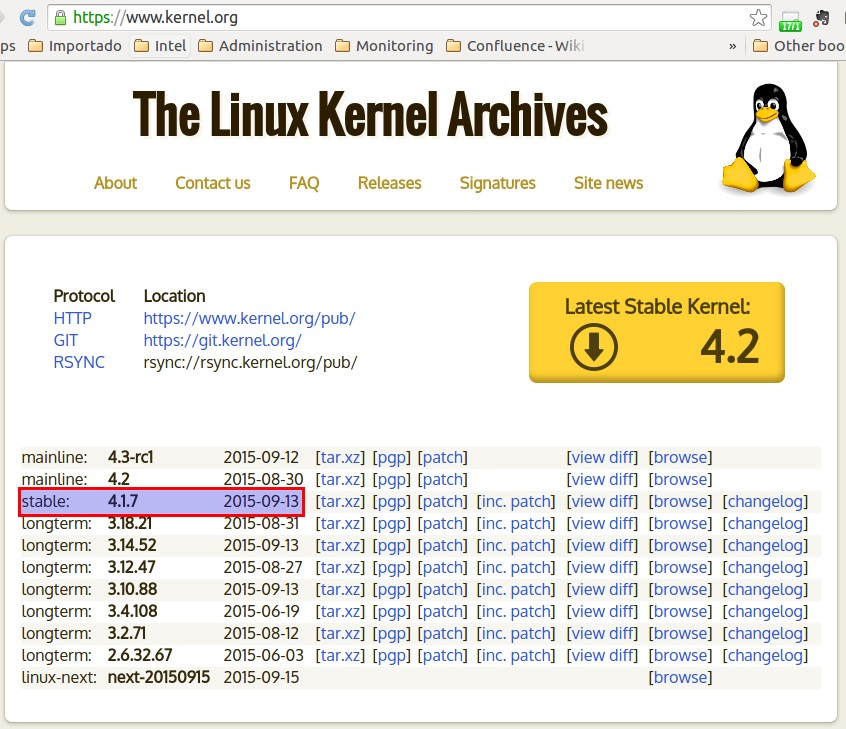
\includegraphics[width=1 \textwidth,
keepaspectratio]{/home/delivery/Desktop/DiploLinuxLatex/Figuras/LinuxKernel.jpg}
\caption{\emph{The Linux Kernel Archives \cite{linuxkernel1}.}}
\end{figure}

\clearpage

\subsubsection{Versión mas usada de kernel estable en \ac{gnu}/Linux}
Considerando que la versión estable 2.6.10 del Kernel de Linux se lanzó en Diciembre del 2003 y aún
esta vigente y en use podemos decir que esta versión estable es la ampliamente desplegada y utilizada.

Versión 2.6, lanzada el	17 December 2003. Versión actual 2.6.32 - 2.6.39
\ac{eol} (maintained from May 2011 to August 2011), last stable release of the 2.6 kernel series.
longterm:	2.6.32.67	2015-06-03

Por su parte, cabe considerar la versión y los releases 3.0 del Kernel ya que esta versión tomó lugar 
el 21 de Julio del 2011 y su último release longterm:3.18.21 (2015-08-31) demostrando una validez de ya
cinco años.

\cite{wikikernel1}

\subsection{Actividad 2.}

\subsubsection{¿De qué distribución deriva \ac{gnu}/Linux Fedora?} 


\emph{``The Fedora Project is a global partnership of free software community members. 
The Fedora Project is sponsored by \textbf{\emph{Red Hat}}, which invests in our infrastructure and resources to 
encourage collaboration and incubate innovative new technologies. Some of these technologies may later 
be integrated into Red Hat products. They are developed in Fedora and produced under a free and open 
sogenurce license from inception, so other free software communities and projects are free to study, adopt, 
and modify them.
Read an overview to learn more about our mission, our community, our governance, and what makes Fedora 
unique. You can also learn about our vision and core values the foundations upon which the project is 
built. We also have information relating to our user base, and the objectives for our technical work.''}

\cite{fedoraproject}

\subsection{Actividad 3.}

\subsubsection{Imprimir pantalla del escritorio \ac{gnome}}

Imprimir pantalla del escritorio \ac{gnome}
y guardar la imagen en el home del usuario dentro de un directorio llamado imagen. 
Cabe mencionar que el usuario es nombrado \textbf{\emph{delivery}}.

\begin{figure}[h!] 
\centering
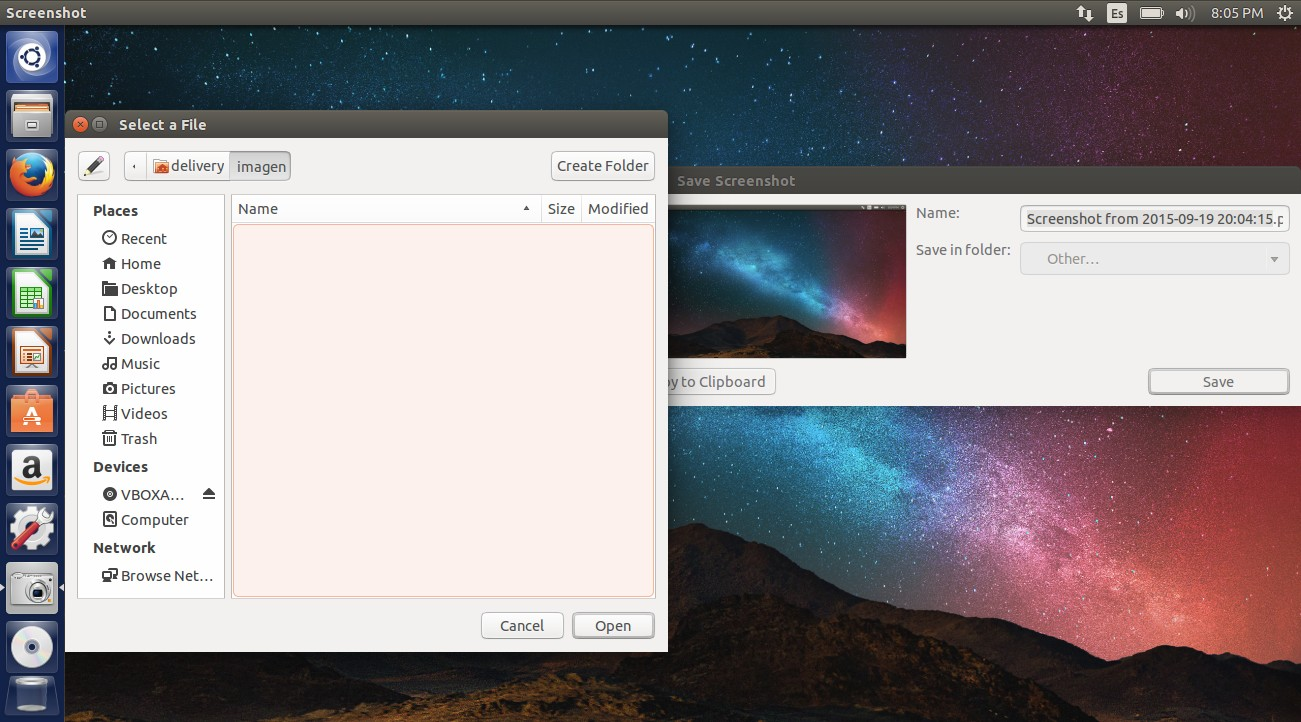
\includegraphics[width=1 \textwidth,
keepaspectratio]{/home/delivery/Desktop/DiploLinuxLatex/Figuras/actividad3.jpg}
\caption{\emph{Capturando pantalla en ubuntu 14.04.}}
\end{figure}

\begin{figure}[h!] 
\centering
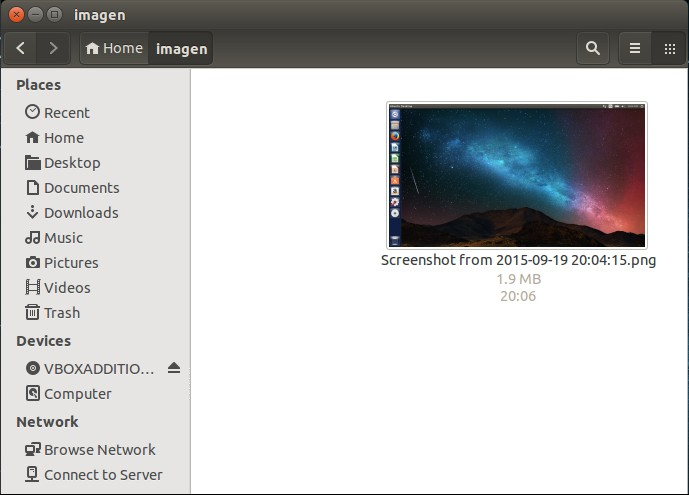
\includegraphics[width=1 \textwidth,
keepaspectratio]{/home/delivery/Desktop/DiploLinuxLatex/Figuras/actividad3b.jpg}
\caption{\emph{Verificando que la captura se haya guardado correctamente en la folder \\ 
/home/delivery/image/.}}
\end{figure}

\pagebreak

\subsection{Actividad 4.}

 \subsubsection{Navegación de directorios con Nautilus}

\textbf{Navegar a través del Nautilus los siguientes directorios:
/home
/etc/
/var/log
/root
/dev
¿En que directorio/s no pudo acceder? ¿Qué tienen de particular los íconos de estos directorios a los que no pudo acceder?\\}

Como usuario sin privilegios a través del navegador de archivos \textbf{\emph{nautilus}}
uno solo podría ingresar y tener control absoluto de los directorios
y archivos dentro de \textbf{\emph{/home}}. Luego con este mismo usuario acceder a \textbf{\emph{/etc, /var/log, /dev}}, pero
sin permisos de escritura o ejecución, solo lectura. Finalmente, el directorio \textbf{\emph{/root}} no es 
accesible a través de la interfaz gráfica ya que no poseemos permisos suficientes para realizar esta
acción. Las carpetas a las cuales carecemos de acceso y permisos se presentan con un candado en el 
icono (considerar que esto no ocurre para el nuevo ubuntu 14.04 como puede verse en las capturas de 
pantalla).

Lo detallado en el párrafo anterior puede apreciarse en las siguientes capturas:

\begin{figure}[h!] 
\centering
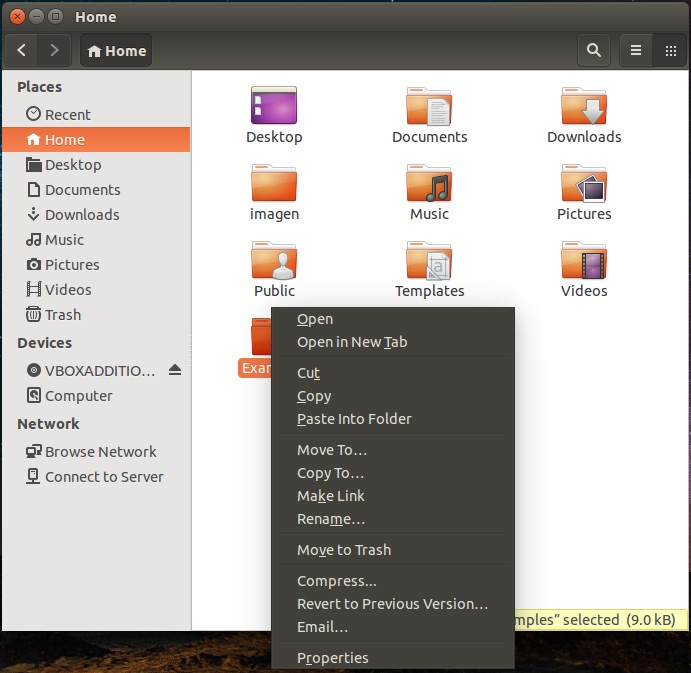
\includegraphics[width=1 \textwidth,
keepaspectratio]{/home/delivery/Desktop/DiploLinuxLatex/Figuras/actividad4a.jpg}
\caption{\emph{Navegación de archivos con Nautius folder: /home .}}
\end{figure}

\begin{figure}[h!] 
\centering
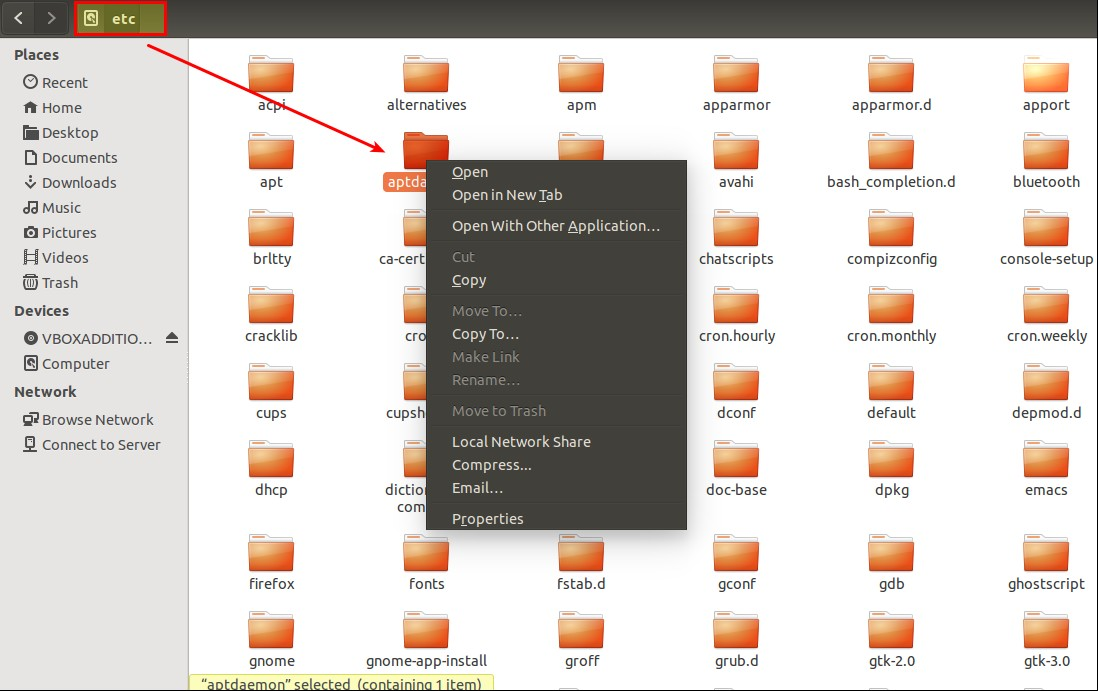
\includegraphics[width=1 \textwidth,
keepaspectratio]{/home/delivery/Desktop/DiploLinuxLatex/Figuras/actividad4b.jpg}
\caption{\emph{Navegación de archivos con Nautius folder: /etc .}}
\end{figure}

\begin{figure}[h!] 
\centering
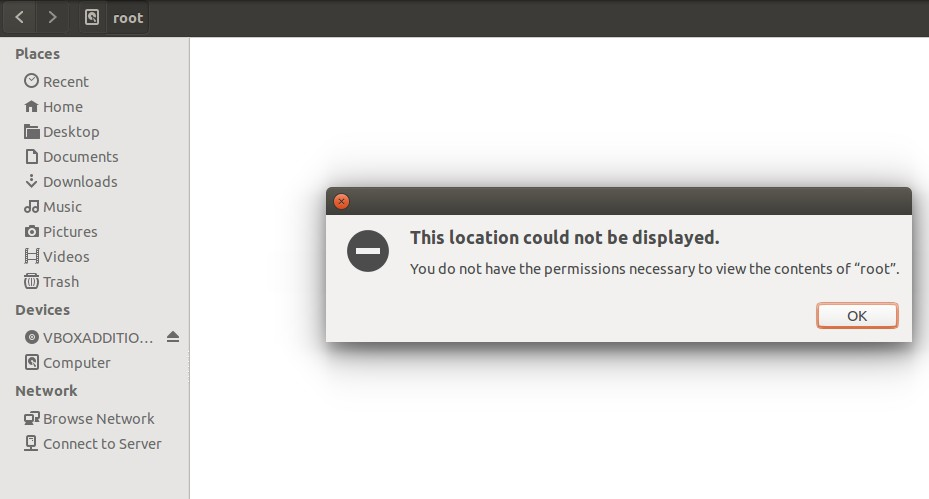
\includegraphics[width=1 \textwidth,
keepaspectratio]{/home/delivery/Desktop/DiploLinuxLatex/Figuras/actividad4c.jpg}
\caption{\emph{Navegación de archivos con Nautius folder: /root.}}
\end{figure}

\clearpage
\pagebreak

\subsection{Actividad 5.}

\subsubsection{LibreOffice Writer: Guardado de archivos .doc en .odt }

\begin{figure}[h!] 
\centering
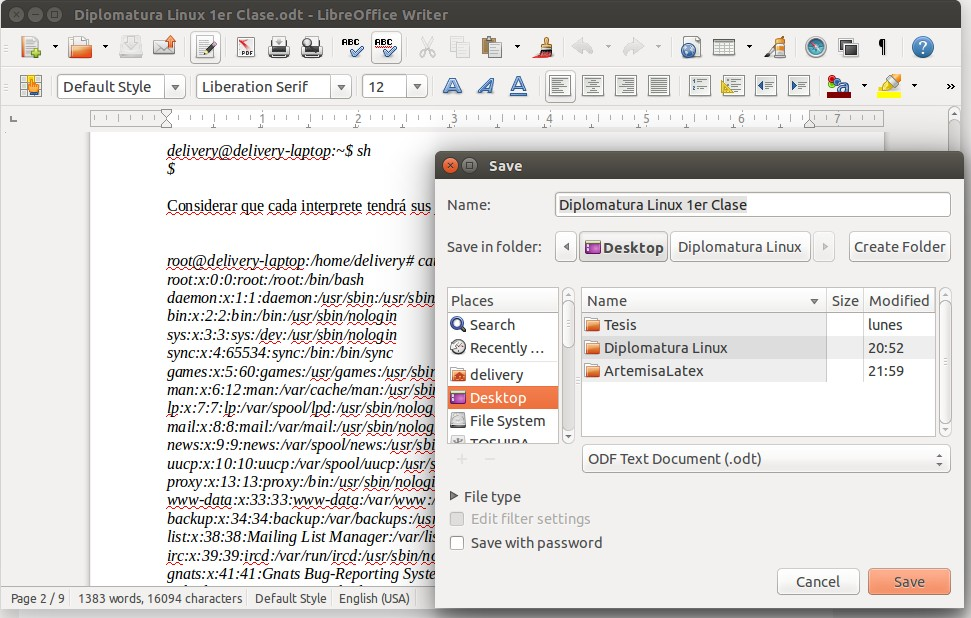
\includegraphics[width=1 \textwidth,
keepaspectratio]{/home/delivery/Desktop/DiploLinuxLatex/Figuras/actividad5.jpg}
\caption{\emph{LibreOffice Writer: Guardado de archivos .doc en .odt.}}
\end{figure}

A un archivo .doc, guardarlo como .odt con LibreOffice Writer.

\pagebreak

\subsection{Actividad 6.}

\subsubsection{Consolas virtuales y \ac{gtk}-Warning}

\textbf{Ejecute la siguiente secuencia de teclas:
Alt+F2 y escriba ``gedit``.
¿Qué sucedió? ¿Qué acción realiza la ejecución de Alt+F2?}\\

Accedemos a la consola virtual número dos. Por su parte no es posible abrir un aplicativo que 
requiere de \ac{gui} para funcionar.

Esto es un evento relacionado a la seguridad de SO normal. Linux es un sistema multiusuario 
donde muchos usuarios podrían estar loggeados, localmente o de forma remota en una sesión GUI.
Luego, ¿qué ocurriría si otros users podrían abrir ventanas en tu escritorio sin su consentimiento?
Claramente esto no sería un comportamiento deseado del SO. Por su parte esto permitiría abrir una 
ventana de gedit u otra aplicación más crítica como un navegador web de forma tal que a este usuario
mal intencionado le permita leer todos nuestros inputs por teclado, pudiendo incluir datos confidenciales
como nuestra cuenta bancaria. Es por esto que se utiliza \textbf{\emph{xhost}} \footnote{NAME:
xhost - server access control program for X. SYNOPSIS: xhost [[+-]name ...] DESCRIPTION: The xhost
program is used to add and delete host names or user names to the list allowed to make connections
to the X server.  In the case of hosts, this provides a rudimentary form of privacy control and security.
It is only sufficient  for  a  workstation  (single user)  environment, although it does limit the
worst abuses.  Environments which require more sophisticated measures should implement
the user-based mechanism or use the hooks in the protocol for passing other authentication data
to the server.\cite{xhost}}.
Por otro lado, la sesión CLI de root no sabe en cual de los displays o pantallas debe abrir la ventana.
Nuevamente cabe remarcar que podría haber varias, tanto locales como remotas. Por lo antedicho surge
la necesidad de declarar la variable de entorno \textbf{\emph{DISPLAY}}. De todas formas existen 
soluciones más prácticas desde la \ac{gui} de usuario normal para manejar estás sesiones,
\textbf{\emph{gnomesu}} en \ac{gnome} y \textbf{\emph{kdesu}} en \ac{kde}. Las cuales básicamente son parte
de una librería para proveer de privilegios de super usuario a las aplicaciones de \ac{gnome}.\\

Cabe mencionar:\\

\emph{''\textbf{Virtual consoles:} In the default Debian system, there are \textbf{six switchable VT100-like character consoles available
to start the command shell directly on the Linux host}. Unless you are in a \ac{gui} environment, 
you can switch between the virtual consoles by \textbf{pressing the Left-Alt-key and one of the F1 — F6
keys simultaneously}. Each character console allows independent login to the account and offers the
multiuser environment. This multiuser environment is a great Unix feature, and very addictive.
If you are under the X Window System, you gain access to the character console 1 by pressing
Ctrl-Alt-F1 key, i.e., the left-Ctrl-key, the left-Alt-key, and the F1-key are pressed together.
You can get back to the X Window System, normally running on the virtual console 7, by pressing Alt-F7.
You can alternatively change to another virtual console, e.g. to the console 1, from the commandline.``}

\texttt{\# chvt 1\\}

\cite{osamu}

\begin{figure}[h!] 
\centering
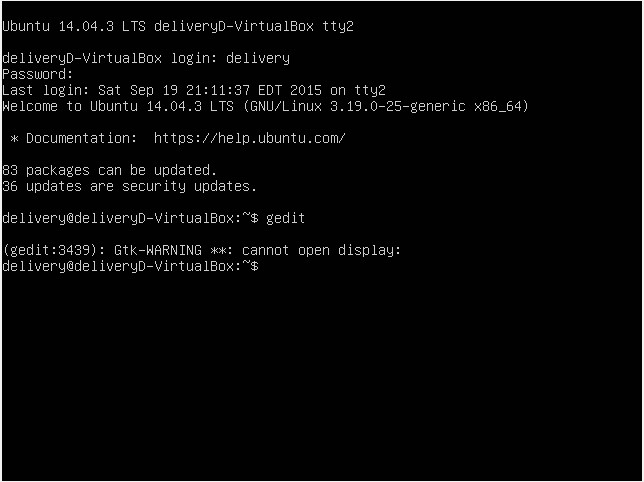
\includegraphics[width=1 \textwidth,
keepaspectratio]{/home/delivery/Desktop/DiploLinuxLatex/Figuras/actividad6.jpg}
\caption{\emph{Linux virtual consoles.}}
\end{figure}

\clearpage
\pagebreak

\section{Ejercicios Tema3: Línea de Comandos. Comandos básicosI }

\begin{itemize}
 \item Concepto de lineas de comando. Presentación de shell bash.
 \item Entender la naturaleza de los privilegios del usuario root.
 \item Moverse y explorar el árbol de jerarquía del Sistema Operativo: ls, cd, mkdir, rmdir.
 \item Copiar, eliminar y renombrar archivos: cp, rm, mv, ln.
 \item Usuarios y permisos: chown, chmod, adduser, addgroup
 \item Crear y ver archivos: touch, less.
\end{itemize}

\subsection{Actividad 1.}

\subsubsection{\ac{cd} command}

\textbf{Desde el directorio /home/curso, cambiar al directorio /etc vía path absoluto. 
Vuelva al directorio /home/curso vía path absoluto.}

\begin{myscriptlisting}
  \begin{verbatim}
delivery@ubuntu:~/curso$ pwd
/home/delivery/curso
delivery@ubuntu:~/curso$ cd /etc/
delivery@ubuntu:/etc$ pwd
/etc
delivery@ubuntu:/etc$ cd /home/delivery/curso/
delivery@ubuntu:~/curso$ pwd
/home/delivery/curso
  \end{verbatim}
\end{myscriptlisting}

\textbf{Repita la acción anterior vía path relativo.
Ejecutar el comando pwd en ambos casos para confirmar el cambio de directorio.}

\begin{myscriptlisting}
  \begin{verbatim}
delivery@ubuntu:~/curso$ pwd
/home/delivery/curso
delivery@ubuntu:~/curso$ cd /etc/
delivery@ubuntu:/etc$ pwd
/etc
delivery@ubuntu:/etc$ cd ~delivery/curso/
delivery@ubuntu:~/curso$ pwd
/home/delivery/curso
  \end{verbatim}
\end{myscriptlisting}

\subsection{Actividad 2.}

\subsubsection{Sudo y permisos de administración}
\textbf{¿Por qué el usuario ``dui`` tiene permisos de administración mientras que el usuario ``curso`` no? 
Algunas pistas:
a.- Revisar a que grupo pertenecen el usuario ``dui`` y ``curso``
b.- Revisar el contenido del archivo /etc/sudoers (archivo de configuración de \ac{sudo})
y ver que permisos tienen los grupos a los cuales pertenecen el usuario ''dui'' y ``curso''.\\}

Se verifican los usuarios creados en el sistema a través del archivo de sistema \textbf{\emph{passwd}} 
donde se encuentran definidas las cuentas de usuario.
Por otro lado, puede verse que el user \textbf{\emph{curso}} no se encuentra en el archivo
\textbf{\emph{sudoers}} por lo que carece de asignación de privilegios de súper usuario a través
del comando \textbf{\emph{\ac{sudo}}}.\\ 

\textbf{NOTA:}
se utilizó el user \textbf{\emph{delivery}} en lugar de \textbf{\emph{dui}}.

\begin{myscriptlisting}
  \begin{verbatim}
curso@ubuntu:~$ cat /etc/passwd | egrep -i 'root|delivery|curso'
root:x:0:0:root:/root:/bin/bash
delivery:x:1000:1000:delivery,,,:/home/delivery:/bin/bash
curso:x:1001:1001:curso,,,:/home/curso:/bin/bash
curso@ubuntu:~$ sudo su
[sudo] password for curso: 
curso is not in the sudoers file.  This incident will be reported.
  \end{verbatim}
\end{myscriptlisting}

Luego con el usuario \textbf{\emph{delivery}} se lee y validan los privilegios
declarados en \textbf{\emph{/etc/sudoers}}. Como ser el user \textbf{\emph{root}}, con permisos 
\textbf{\emph{ALL=(ALL:ALL) ALL}} (se detallará debajo su significado) y los más relevante
para esta práctica revisar que se incluye una línea para permitir a todos los miembros
del grupo \textbf{\emph{\ac{sudo}}} para ejecutar cualquier comando:

\begin{verbatim}
# Allow members of group sudo to execute any command
%sudo	ALL=(ALL:ALL) ALL
\end{verbatim}

\begin{myscriptlisting}
  \begin{verbatim}
curso@ubuntu:~$ su - delivery 
Password: 
delivery@ubuntu:~$ sudo cat /etc/sudoers

#
# This file MUST be edited with the 'visudo' command as root.
#
# Please consider adding local content in /etc/sudoers.d/ instead of
# directly modifying this file.
#
# See the man page for details on how to write a sudoers file.
#
Defaults	env_reset
Defaults	mail_badpass
Defaults	secure_path=``/usr/local/sbin:/usr/local/bin:/usr/sbin:/usr/bin:/sbin:/bin``

# Host alias specification

# User alias specification

# Cmnd alias specification

# User privilege specification
root	ALL=(ALL:ALL) ALL

# Members of the admin group may gain root privileges
%admin ALL=(ALL) ALL

# Allow members of group sudo to execute any command
%sudo	ALL=(ALL:ALL) ALL

# See sudoers(5) for more information on ``#include`` directives:

#includedir /etc/sudoers.d
  \end{verbatim}
\end{myscriptlisting}

Finalmente se verifica en \textbf{\emph{/etc/group}} lo comentado anteriormente
donde el user \textbf{\emph{delivery}} pertenece al grupo \ac{sudo} con \textbf{\emph{GID = 27}}
y el user \textbf{\emph{curso}} no.

\begin{myscriptlisting}
  \begin{verbatim}
delivery@ubuntu:~$ cat /etc/group | egrep -i 'curso|delivery|root'
root:x:0:
adm:x:4:syslog,delivery
cdrom:x:24:delivery
sudo:x:27:delivery
dip:x:30:delivery
plugdev:x:46:delivery
delivery:x:1000:
lpadmin:x:110:delivery
sambashare:x:111:delivery
curso:x:1001:
  \end{verbatim}
\end{myscriptlisting}


\textbf{Sudo} is a program designed to let system administrators allow some users to execute some commands
as root (or another user). The basic philosophy is to give as few privileges as possible but still
allow people to get their work done. \ac{sudo} is also an effective way to log who ran which command and when.

As of most Debian based distributions, if you ask for the Desktop task during the installation, that pulls in \ac{sudo} with
a default configuration that automatically grants sudo-ing rights to any member of the \ac{sudo} group.
Depending on what user accounts you set up during the install, it's still possible that you may not
have been added to that group - you can check by running groups.\\

\textbf{Why \ac{sudo}?}
Using sudo is better (safer) than opening a session as root for a number of reasons, including:
\begin{enumerate}
 \item Nobody needs to know the root password (\ac{sudo} prompts for the current user's password). 
 Extra privileges can be granted to individual users temporarily, and then taken away without the 
 need for a password change.
 
 \item It's easy to run only the commands that require special privileges via \ac{sudo}; the rest of the time,
you work as an unprivileged user, which reduces the damage that mistakes can cause.
Auditing/logging: when a \ac{sudo} command is executed, the original username and the command are logged.
 
 \item For the reasons above, switching to root using \ac{sudo} -i (or sudo su) is usually deprecated because
it cancels the above features.

\end{enumerate}

Sudo is a program designed to allow a sysadmin to give limited root privileges to users and log root
activity. The basic philosophy is to give as few privileges as possible but still allow people to get
their work done.\\

\cite{debiansudo}

\%sudo ALL=(ALL) ALL
\begin{itemize}
 \item \textbf{\%sudo} the group named "admin" (\% prefix) is the group or users that
 are receiving the permises.
 \item \textbf{ALL=} The 2nd parameter refers to the host where the before mentioned group or
 users will have priviledges. For this exampe in ALL hosts (this will work if you distribute
 the same sudoers file to many computers, or if someone access remotely - however no recommended
 from a secutiry point of view).
 \item \textbf{(ALL)} The third one is the user as you are running the command. In this case
 as any target user.
 \item \textbf{ALL} The last one is the commands allowed. So the users in sudo group, in any host
 as any user including root, can run any command.
\end{itemize}

\subsection{Actividad 3.}

\subsubsection{less command}
\textbf{Revisar con el comando "less" el contenido del archivo /etc/passwd y en él buscar a los usuarios 
root, curso y dui}

\begin{myscriptlisting}
  \begin{verbatim}
delivery@ubuntu:~$ less /etc/passwd | egrep 'root|curso|delivery'
root:x:0:0:root:/root:/bin/bash
delivery:x:1000:1000:delivery,,,:/home/delivery:/bin/bash
curso:x:1001:1001:curso,,,:/home/curso:/bin/bash
  \end{verbatim}
\end{myscriptlisting}

\subsection{Actividad 4.}

\subsubsection{/bin and /sbin}
\textbf{¿Cuál es la diferencia entre los directorios /bin y /sbin?}

\begin{itemize}
 \item \textbf{/bin}\\
    This directory contains executable programs which are needed
    in single user mode and to bring the system up or repair it.
\end{itemize}

\begin{mytinylisting}
 \begin{verbatim}
delivery@ubuntu:/sbin$ cd /bin
delivery@ubuntu:/bin$ pwd
/bin
delivery@ubuntu:/bin$ ls
bash          chvt                  fgconsole   lesspipe    nc                ntfstruncate             sed     
bunzip2       cp                    fgrep       ln          nc.openbsd        ntfswipe                 setfacl          
busybox       cpio                  findmnt     loadkeys    netcat            open                     setfont          
bzcat         dash                  fuser       login       netstat           openvt                   setupcon         
bzcmp         date                  fusermount  loginctl    nisdomainname     pidof                    sh               
bzdiff        dbus-cleanup-sockets  getfacl     lowntfs-3g  ntfs-3g           ping                     sh.distrib       
bzegrep       dbus-daemon           grep        ls          ntfs-3g.probe     ping6                    sleep            
bzexe         dbus-uuidgen          gunzip      lsblk       ntfs-3g.secaudit  plymouth                 ss               
bzfgrep       dd                    gzexe       lsmod       ntfs-3g.usermap   plymouth-upstart-bridge  static-sh        
bzgrep        df                    gzip        mkdir       ntfscat           ps                       stty             
bzip2         dir                   hostname    mknod       ntfsck            pwd                      su               
bzip2recover  dmesg                 ip          mktemp      ntfscluster       rbash                    sync             
bzless        dnsdomainname         kbd_mode    more        ntfscmp           readlink                 tailf            
bzmore        domainname            kill        mount       ntfsdump_logfile  red                      tar              
cat           dumpkeys              kmod        mountpoint  ntfsfix           rm                       tempfile         
chacl         echo                  less        mt          ntfsinfo          rmdir                    touch            
chgrp         ed                    lessecho    mt-gnu      ntfsls            rnano                    true             
chmod         egrep                 lessfile    mv          ntfsmftalloc      running-in-container     udevadm          
chown         false                 lesskey     nano        ntfsmove          run-parts       
 \end{verbatim}
\end{mytinylisting}    

\begin{itemize}

\item \textbf{/sbin}\\
    Like /bin, this directory holds commands needed to boot the 
    system, but which are usually not executed by normal users.
\end{itemize}

\begin{mytinylisting}
 \begin{verbatim}
delivery@ubuntu:/sbin$ ls
acpi_available   e2fsck        fstrim-all         iptables-apply    mkfs.bfs          nameif        rmmod                    
agetty           e2image       gdisk              iptables-restore  mkfs.cramfs       ntfsclone     route                    
alsa             e2label       getcap             iptables-save     mkfs.ext2         ntfscp        rtacct                   
apm_available    e2undo        getpcaps           iptunnel          mkfs.ext3         ntfslabel     rtmon                    
apparmor_parser  ethtool       getty              isosize           mkfs.ext4         ntfsresize    runlevel                 
badblocks        fatlabel      halt               iwconfig          mkfs.ext4dev      ntfsundelete  setcap                   
biosdevname      fdisk         hdparm             iwevent           mkfs.fat          on_ac_power   setvtrgb                 
blkid            findfs        hwclock            iwgetid           mkfs.minix        pam_tally     sfdisk                   
blockdev         fixparts      ifconfig           iwlist            mkfs.msdos        pam_tally2    sgdisk                   
bridge           fsck          ifdown             iwpriv            mkfs.ntfs         parted        shadowconfig             
capsh            fsck.cramfs   ifquery            iwspy             mkfs.vfat         partprobe     shutdown                 
cfdisk           fsck.ext2     ifup               kbdrate           mkhomedir_helper  pivot_root    slattach                 
cgdisk           fsck.ext3     init               killall5          mkntfs            plipconfig    start                    
crda             fsck.ext4     initctl            ldconfig          mkswap            plymouthd     startpar                 
ctrlaltdel       fsck.ext4dev  insmod             ldconfig.real     mntctl            poweroff      startpar-upstart-inject  
debugfs          fsck.fat      installkernel      logsave           modinfo           rarp          start-stop-daemon        
depmod           fsck.minix    ip                 losetup           modprobe          raw           status                   
dhclient         fsck.msdos    ip6tables          lsmod             mountall          reboot        stop                     
dhclient-script  fsck.nfs      ip6tables-apply    MAKEDEV           mount.fuse        regdbdump     sulogin                  
dmsetup          fsck.vfat     ip6tables-restore  mii-tool          mount.lowntfs-3g  reload        swaplabel                
dosfsck          fsfreeze      ip6tables-save     mkdosfs           mount.ntfs        resize2fs     swapoff                  
dosfslabel       fstab-decode  ipmaddr            mke2fs            mount.ntfs-3g     resolvconf    swapon
dumpe2fs         fstrim        iptables           mkfs              mount.vboxsf      restart       switch_root
 \end{verbatim}
\end{mytinylisting}

Directorios relacionados:
    
\begin{itemize}
 \item \textbf{/usr/bin}\\   
    This is the primary directory for executable programs. Most
    programs executed by normal users which are not needed for 
    booting or for repairing the system and which are not
    installed locally should be placed in this directory.

\item \textbf{/usr/local}\\
    This is where programs which are local to the site typically
    go.
    
 \item \textbf{/usr/local}\\
    This is where programs which are local to the site typically
    go.
    
 \item \textbf{/usr/local/bin}\\
    Binaries for programs local to the site.
 
  \item \textbf{/usr/local/sbin}\\
    Locally installed programs for system administration.
\end{itemize}

\cite{wikifhs}

\subsection{Actividad 5.}

\subsubsection{Listado de permisos ''ls -la`` command}
\textbf{Liste el contenido del directorio /home/curso (incluido los archivos ocultos). 
Se requiere saber el permiso de acceso, dueño y grupo de cada archivo del directorio.}

\begin{myscriptlisting}
  \begin{verbatim}
delivery@ubuntu:~$ cd /home/delivery/
delivery@ubuntu:~$ pwd
/home/delivery
delivery@ubuntu:~$ ls -la
total 128
drwxr-xr-x 19 delivery delivery 4096 Sep 20 19:54 .
drwxr-xr-x  4 root     root     4096 Sep 20 19:49 ..
-rw-------  1 delivery delivery 1295 Sep 20 19:38 .bash_history
-rw-r--r--  1 delivery delivery  220 Sep 16 10:17 .bash_logout
-rw-r--r--  1 delivery delivery 3637 Sep 16 10:17 .bashrc
drwx------ 14 delivery delivery 4096 Sep 20 19:54 .cache
drwx------  3 delivery delivery 4096 Sep 20 14:03 .compiz
drwx------ 17 delivery delivery 4096 Sep 20 19:54 .config
drwxrwxr-x  2 delivery delivery 4096 Sep 20 19:41 curso
drwx------  3 delivery delivery 4096 Sep 20 17:56 .dbus
drwxr-xr-x  2 delivery delivery 4096 Sep 19 21:11 Desktop
drwxrwxr-x  3 delivery delivery 4096 Sep 20 19:12 DiploLinux
-rw-r--r--  1 delivery delivery   33 Sep 20 14:03 .dmrc
drwxr-xr-x  2 delivery delivery 4096 Sep 19 21:11 Documents
drwxr-xr-x  2 delivery delivery 4096 Sep 19 21:11 Downloads
drwx------  3 delivery delivery 4096 Sep 20 17:56 .gconf
-rw-------  1 delivery delivery 1590 Sep 20 17:56 .ICEauthority
drwx------  3 delivery delivery 4096 Sep 19 21:11 .local
drwxr-xr-x  2 delivery delivery 4096 Sep 19 21:11 Music
drwxr-xr-x  2 delivery delivery 4096 Sep 19 21:11 Pictures
drwx------  3 delivery delivery 4096 Sep 20 19:54 .pki
-rw-r--r--  1 delivery delivery  675 Sep 16 10:17 .profile
drwxr-xr-x  2 delivery delivery 4096 Sep 19 21:11 Public
drwxr-xr-x  2 delivery delivery 4096 Sep 19 21:11 Templates
-rw-r-----  1 delivery delivery    5 Sep 20 17:56 .vboxclient-clipboard.pid
-rw-r-----  1 delivery delivery    5 Sep 20 17:56 .vboxclient-display.pid
-rw-r-----  1 delivery delivery    5 Sep 20 17:56 .vboxclient-draganddrop.pid
-rw-r-----  1 delivery delivery    5 Sep 20 17:56 .vboxclient-seamless.pid
drwxr-xr-x  2 delivery delivery 4096 Sep 19 21:11 Videos
-rw-------  1 delivery delivery   51 Sep 20 17:56 .Xauthority
-rw-------  1 delivery delivery  908 Sep 20 17:56 .xsession-errors
-rw-------  1 delivery delivery 1294 Sep 20 17:14 .xsession-errors.old
  \end{verbatim}
\end{myscriptlisting}

\textbf{Permisos a archivos}
Para permitir establecer los permisos en un archivo contamos con el comando chmod.
Este comando funciona con la siguiente sintaxis:\\

\texttt{Chmod [opciones] permisos archivo/directorio}\\

Antes de adentrarnos en el comando es necesario explicar algunas cosas. Tenemos dos
maneras de asignar permisos a los usuarios, mediante un modo octal y modo carácter.\\

\textbf{Modo Octal}
El modo octal responde a la combinación de los tres permisos con las tres clases de
usuario formando un numero binario de 3 cifras donde:

\begin{itemize}
 \item El primer digito corresponde a los permisos del dueño
 \item El segundo a los del grupo
 \item El tercero al resto de los usuarios
\end{itemize}

La instrucción quedaría asi:\\
\texttt{chmod 760 archivo.txt}\\

\textbf{Modo carácter}
Posee 3 modificadores que permiten realizar la tarea:
\begin{itemize}
 \item + : añade un modo
 \item – : elimina un modo
 \item = : específica un modo (sobrescribiendo el anterior)
\end{itemize}

Los modos son \textbf{r (read), w (write), x(ejecutar)}. y los usuarios están representados por:
\begin{itemize}
 \item u: dueño
 \item g: grupo
 \item o : otros
 \item a : todos
\end{itemize}

Entonces si quiero agregar el permiso de escribir a todos, escribo:\\
\texttt{chmod a+w archivo.txt}\\

\cite{mirizioe}

\subsection{Actividad 6.}

\subsubsection{Listado de permisos ''ls -l`` command}
\textbf{Liste el contenido del directorio /etc. Debe aparecer cada archivo contenido en una 
linea aparte sin detalles de permisos de acceso, dueño o grupo.}

\begin{myscriptlisting}
  \begin{verbatim}
delivery@ubuntu:/etc$ pwd
/etc
delivery@ubuntu:/etc$ ls -1
acpi
adduser.conf
alternatives
anacrontab
apg.conf
apm
apparmor
apparmor.d
apport
apt
at.deny
at-spi2
avahi
bash.bashrc
bash_completion
bash_completion.d
bindresvport.blacklist
blkid.conf
blkid.tab
bluetooth
...
update-manager
update-motd.d
update-notifier
UPower
upstart-xsessions
vim
vtrgb
w3m
wgetrc
wodim.conf
wpa_supplicant
X11
xdg
xml
zsh_command_not_found
  \end{verbatim}
\end{myscriptlisting}

\subsection{Actividad 7.}

\subsubsection{mkdir make directory}
\textbf{Cree en el directorio /home/curso la siguiente estructura de directorio}

\begin{verbatim}
./raiz
|___bin
|___home
| |___ApellidoNombre
| |___Desktop
| |___bin
|___var
..|__log
\end{verbatim}

\begin{verbatim}
curso@ubuntu:~$ pwd
/home/curso
curso@ubuntu:~$ mkdir ./raiz ./raiz/bin ./raiz/home ./raiz/home/BarrireroExequiel
./raiz/home/Desktop ./raiz/home/bin ./raiz/var ./raiz/var/log  

curso@ubuntu:~$ ls -R
.:
raiz

./raiz:
bin  home  var

./raiz/bin:

./raiz/home:
BarrireroExequiel  bin  Desktop

./raiz/home/BarrireroExequiel:

./raiz/home/bin:

./raiz/home/Desktop:

./raiz/var:
log

./raiz/var/log:
\end{verbatim}

\textbf{¿Qué significa ./?}\\
Refiere a \textbf\emph{{''este directorio``}}, es decir al directorio actual en el que nos
encontramos posicionados en la terminal.

\subsection{Actividad 8.}

\subsubsection{Creación de archivos con ''touch``}
\textbf{Sobre el esquema de directorios creado en la Actividad 7, cree con
``touch`` un archivo en /home/curso/raiz/var/log/messages}

\begin{verbatim}
 curso@ubuntu:~$ touch /home/curso/raiz/var/log/messages
curso@ubuntu:~$ ls -la /home/curso/raiz/var/log/
total 8
drwxrwxr-x 2 curso curso 4096 Sep 29 18:58 .
drwxrwxr-x 3 curso curso 4096 Sep 20 22:38 ..
-rw-rw-r-- 1 curso curso    0 Sep 29 18:57 messages
\end{verbatim}

\subsection{Actividad 9.}

\subsubsection{Cambio de permisos con ''chmod``}
\textbf{Liste con ``ls`` los permisos de acceso del archivo creado en la Actividad 8.
Luego con ``chmod`` cambie los permisos de acceso del archivo creado en la Actividad 8 
a rwx solo para el grupo.}

\begin{verbatim}
curso@ubuntu:~$ ls -la /home/curso/raiz/var/log/
total 8
drwxrwxr-x 2 curso curso 4096 Sep 29 18:58 .
drwxrwxr-x 3 curso curso 4096 Sep 20 22:38 ..
-rw-rw-r-- 1 curso curso    0 Sep 29 18:57 messages
curso@ubuntu:~$ chmod g+rwx /home/curso/raiz/var/log/messages 
curso@ubuntu:~$ ls -la /home/curso/raiz/var/log/
total 8
drwxrwxr-x 2 curso curso 4096 Sep 29 18:58 .
drwxrwxr-x 3 curso curso 4096 Sep 20 22:38 ..
-rw-rwxr-- 1 curso curso    0 Sep 29 18:57 messages 
\end{verbatim}

\subsection{Actividad 10.}

\subsubsection{Eliminar recursivamente con ''rm`` command}
\textbf{Elimine recursivamente el directorio ``/home/curso/raiz/var``}

\begin{verbatim}
curso@ubuntu:~$ rm -r /home/curso/raiz/var/
curso@ubuntu:~$ ll /home/curso/raiz/
total 16
drwxrwxr-x  4 curso curso 4096 Sep 29 19:07 ./
drwxr-xr-x 17 curso curso 4096 Sep 29 19:02 ../
drwxrwxr-x  2 curso curso 4096 Sep 20 22:38 bin/
drwxrwxr-x  5 curso curso 4096 Sep 20 22:38 home/
\end{verbatim}

\subsection{Actividad 11.}

\subsubsection{Copia recursiva de directorio con ''cp`` command}
\textbf{Cree el directorio /home/curso/raiz/etc. 
Luego copie TODO el contenido del directorio /etc/ dentro de /home/curso/raiz/etc}

\begin{myscriptlisting}
  \begin{verbatim}
 curso@ubuntu:~$ mkdir /home/curso/raiz/etc
curso@ubuntu:~$ cp /etc/* /home/curso/raiz/etc/

curso@ubuntu:~$ sudo cp -R /etc/* /home/curso/raiz/etc/ 
curso@ubuntu:~$ ls -l /home/curso/raiz/etc/
total 1016
drwxr-xr-x  3 root  root   4096 Sep 29 19:21 acpi
-rw-r--r--  1 curso curso  2981 Sep 29 19:21 adduser.conf
drwxr-xr-x  2 root  root   4096 Sep 29 19:21 alternatives
-rw-r--r--  1 curso curso   401 Sep 29 19:21 anacrontab
-rw-r--r--  1 curso curso   112 Sep 29 19:21 apg.conf
drwxr-xr-x  6 root  root   4096 Sep 29 19:21 apm
drwxr-xr-x  3 root  root   4096 Sep 29 19:21 apparmor
drwxr-xr-x  8 root  root   4096 Sep 29 19:21 apparmor.d
drwxr-xr-x  4 root  root   4096 Sep 29 19:21 apport
drwxr-xr-x  6 root  root   4096 Sep 29 19:21 apt
-rw-r-----  1 root  root    144 Sep 29 19:21 at.deny
drwxr-xr-x  2 root  root   4096 Sep 29 19:21 at-spi2
drwxr-xr-x  3 root  root   4096 Sep 29 19:21 avahi
-rw-r--r--  1 curso curso  2177 Sep 29 19:21 bash.bashrc
-rw-r--r--  1 curso curso    45 Sep 29 19:21 bash_completion
drwxr-xr-x  2 root  root   4096 Sep 29 19:21 bash_completion.d
-rw-r--r--  1 curso curso   356 Sep 29 19:21 bindresvport.blacklist
-rw-r--r--  1 curso curso   321 Sep 29 19:21 blkid.conf
lrwxrwxrwx  1 root  root     15 Sep 29 19:21 blkid.tab -> /dev/.blkid.tab
drwxr-xr-x  2 root  root   4096 Sep 29 19:21 bluetooth
drwxr-xr-x  2 root  root   4096 Sep 29 19:21 bonobo-activation
drwxr-xr-x  2 root  root   4096 Sep 29 19:21 byobu
drwxr-xr-x  3 root  root   4096 Sep 29 19:21 ca-certificates
...
-rw-r--r--  1 curso curso   321 Sep 29 19:21 updatedb.conf
drwxr-xr-x  3 root  root   4096 Sep 29 19:21 update-manager
drwxr-xr-x  2 root  root   4096 Sep 29 19:21 update-motd.d
drwxr-xr-x  2 root  root   4096 Sep 29 19:21 update-notifier
drwxr-xr-x  2 root  root   4096 Sep 29 19:21 UPower
-rw-r--r--  1 curso curso   222 Sep 29 19:21 upstart-xsessions
drwxr-xr-x  2 root  root   4096 Sep 29 19:21 vim
lrwxrwxrwx  1 root  root     23 Sep 29 19:21 vtrgb -> /etc/alternatives/vtrgb
drwxr-xr-x  2 root  root   4096 Sep 29 19:21 w3m
-rw-r--r--  1 curso curso  4812 Sep 29 19:21 wgetrc
-rw-r--r--  1 curso curso  1343 Sep 29 19:21 wodim.conf
drwxr-xr-x  2 root  root   4096 Sep 29 19:21 wpa_supplicant
drwxr-xr-x 10 root  root   4096 Sep 29 19:21 X11
drwxr-xr-x  4 root  root   4096 Sep 29 19:21 xdg
drwxr-xr-x  2 root  root   4096 Sep 29 19:21 xml
-rw-r--r--  1 curso curso   349 Sep 29 19:21 zsh_command_not_found
  \end{verbatim}
\end{myscriptlisting}

\textbf{NOTA:}
man for ''cp`` command

\begin{verbatim}
CP(1)                                                                      

NAME
       cp - copy files and directories

SYNOPSIS
       cp [OPTION]... [-T] SOURCE DEST
       cp [OPTION]... SOURCE... DIRECTORY
       cp [OPTION]... -t DIRECTORY SOURCE...

DESCRIPTION
       Copy SOURCE to DEST, or multiple SOURCE(s) to DIRECTORY.
...       
       -R, -r, --recursive
              copy directories recursively
...
\end{verbatim}

\subsection{Actividad 12.}

\subsubsection{Renombrar archivos con ''mv`` command}
\textbf{Renombre con ``mv`` el directorio /home/curso/raiz por /home/curso/root}

\begin{myscriptlisting}
 \begin{verbatim}
curso@ubuntu:~$ ls -ls /home/curso/
total 2008
   4 drwxrwxr-x 3 curso curso    4096 Sep 21 19:25 BarrireroExequiel
1968 -rw-rw-r-- 1 curso curso 2013003 Sep 21 21:13 BarrireroExequiel.tar.gz
   4 drwxr-xr-x 2 curso curso    4096 Sep 29 19:18 Desktop
   4 drwxr-xr-x 2 curso curso    4096 Sep 21 14:06 Documents
   4 drwxr-xr-x 2 curso curso    4096 Sep 21 19:30 Downloads
   4 drwxr-xr-x 2 curso curso    4096 Sep 21 14:06 Music
   4 drwxr-xr-x 2 curso curso    4096 Sep 21 20:53 Pictures
   4 drwxr-xr-x 2 curso curso    4096 Sep 21 14:06 Public
   4 drwxrwxr-x 5 curso curso    4096 Sep 29 19:20 root
   4 drwxr-xr-x 2 curso curso    4096 Sep 21 14:06 Templates
   4 drwxr-xr-x 2 curso curso    4096 Sep 21 14:06 Videos

curso@ubuntu:~$ ls -ls /home/curso/ | grep root
   4 drwxrwxr-x 5 curso curso    4096 Sep 29 19:20 root
 \end{verbatim}
\end{myscriptlisting}


\subsection{Actividad 13.}

\subsubsection{Copia de dirs mediante path relativo}
\textbf{Copie el directorio /home/curso/root/var/log a /home/curso/root/var/log.original
utilizando PATH relativo desde /home/curso}

\begin{myscriptlisting}
 \begin{verbatim}
curso@ubuntu:~$ pwd
/home/curso
curso@ubuntu:~$ cp -R ./root/var/log/ ./root/var/log.original

curso@ubuntu:~$ pwd
/home/curso
curso@ubuntu:~$ ls ./root/var/
log  log.original

curso@ubuntu:~$ ls -la ./root/var/
total 16
drwxrwxr-x 4 curso curso 4096 Sep 29 19:44 .
drwxrwxr-x 6 curso curso 4096 Sep 29 19:42 ..
drwxrwxr-x 2 curso curso 4096 Sep 29 19:42 log
drwxrwxr-x 2 curso curso 4096 Sep 29 19:44 log.original
 \end{verbatim}
\end{myscriptlisting}

\subsection{Actividad 14.}

\subsubsection{Enlaces simbólicos ''ln'' command}
\textbf{Cree un link simbólico de /etc/group en /home/curso}

\begin{myscriptlisting}
 \begin{verbatim}
curso@ubuntu:~$ ln -s /etc/group /home/curso/
curso@ubuntu:~$ ls -la /home/curso/ | grep group
lrwxrwxrwx  1 curso curso      10 Sep 29 19:55 group -> /etc/group

curso@ubuntu:~$ ls -i /home/curso/ | grep group 
533568 group
curso@ubuntu:~$ ls -i /etc/ | grep group
418231 group
 \end{verbatim}
\end{myscriptlisting}


\textbf{Enlaces de Ficheros \\}

Los enlaces ofrecen la posibibilidad de dar a un único fichero múltiples nombres. 
Estos ficheros van a ser identificados mediante el sistema operativo por su numero de inodo, 
el cual se genera de forma semialeatoria. Solo para ficheros y sólo en particiones linux.

Un inodo es un enlace que resulta el único identificador del fichero para el sistema de ficheros.
Un directorio, por tanto, será una lista de números de inodo con sus correspondientes nombres de fichero.
Cada nombre de fichero en un directorio es un enlace a un inodo particular.

\begin{itemize}
 \item \textbf{\emph{Enlaces Duros o hard links:}}
 
 La orden ln es usada para crear enlaces para un fichero.

Usando \texttt{ls -i}, veremos el numero de inodo para el fichero.

\# \texttt{ln fichero} creará un enlace para fichero.

\texttt{ln fichero fhichero2} creará un enlace llamado fichero2 que corresponderá al mismo fichero.

Utilizando \texttt{ls -i} veremos que los dos ficheros tienen el mismo inodo.

\# \texttt{ls -i fichero fichero2}

Un fichero estará definitivamente eliminado del sistema cuando no queden enlaces a el. En realidad,
la norma es que los ficheros tengan solamente un enlace duro.

Un modo de saber cuantos enlaces tiene un fichero es con la orden \texttt{ls -l}. 
Fíjate en la salida estándar por pantalla, la primera columna indica los permisos, 
como vimos en lecciones pasadas, y una segunda columna con un número te indicará el número 
de enlaces del fichero, o, si es un directorio, el número de directorios que contiene, 
en nuestro ejemplo te mostraría lo siguiente:

\texttt{ls -l fichero fichero2}

\texttt{-rw-r-r- 2 root root 12 Aug 5 16:51 fichero}

\texttt{-rw-r-r- 2 root root 12 Aug 5 16:50 fichero2}

un directorio, por tanto, no es otra cosa que un fichero que contiene información sobre la
dirección del enlace al inodo. También, cada directorio tiene al menos dos enlaces duros en 
el: . (punto) enlace que apunta a si mismo y .. (punto punto) enlace que apunta al directorio padre.
En el directorio raíz (/), el enlace .. (punto punto) simplemente apunta a /.

\textbf{Buscar todos los enlaces duros a un fichero.}
En ciertas ocasiones puede resultar difícil localizar en que partes del árbol de directorio
existen enlaces a determinados archivos. Para encontrarlos lo podemos hacer con la orden find:
\texttt{find / -inum número}

\item \textbf{\emph{Enlaces Simbólicos}}

Un enlace simbólico permite dar a un fichero el nombre de otro, pero no enlaza el fichero con un inodo,
es decir, en realidad lo que hacemos es enlazar directamente al nombre del fichero. 
Esto podría parecerse bastante a lo que Windows nos tiene acostumbrados.

Con la orden \texttt{ln -s} creamos un enlace simbólico a un fichero. Por ejemplo:

\texttt{ln -s archivo archivo2}

Hay que tener en cuenta que el nombre del enlace simbólico no soporta rutas completas, 
por lo que para crearlo, será imprescindible situarse dentro del directorio en el que queramos
que quede colocado dicho enlace.

Si lo verificamos de nuevo con la orden \texttt{ls -l} vemos que el fichero fichero es 
un enlace simbólico apuntando a fichero2

\texttt{ls -l fichero fichero2}

Los bits de permisos en un enlace simbólico no se usan (siempre aparecen como (rwxrwxrwx).
En su lugar, los permisos del enlace simbólico son determinados por los permisos del fichero apuntado. 
Asimismo, si el fichero apuntado es eliminado, los enlaces simbólicos permanecen, pero ya no 
serán válidos y carecerán de sentido.
\end{itemize}

Los enlaces duros y simbólicos son similares en su funcionamiento, pero hay algunas diferencias. 
Pueden crearse enlaces simbólicos a un fichero que no esté en el mismo dispositivo de almacenamiento.
Los enlaces simbólicos son procesados por el núcleo de forma diferente a los duros, lo cual es solo
una diferencia técnica, pero a veces importante. Los enlaces simbólicos son de ayuda puesto que
identifican al fichero al que apuntan; con enlaces duros no es tan fácil saber que fichero esta
enlazado al mismo inodo.

Aunque en un principio no pudiera parecernos que los enlaces valgan para mucho, el sistema
operativo los usa muy a menudo, Los enlaces simbólicos son, por ejemplo, especialmente
importantes para las imágenes de las librerías compartidas en /lib, lo que facilita mucho la
conexión de los diferentes programas con esas librerías.

\cite{utlai}


\subsection{Actividad 15.}

\subsubsection{Navegación de directorios con Nautilus}
\textbf{Luego de la ejecución de un comando ls -l ¿Qué significa el número que se 
encuentra entre el listado de permisos y el nombre del usuario dueño?\\ \\
\texttt{curso@atlas:~> ls –l}\\ 
\texttt{-rwx------ 1 curso curso 11 2011-05-11 23:56 password}}\\

Un modo de saber cuantos enlaces tiene un fichero es con la orden \texttt{ls -l}. 
Fíjate en la salida estándar por pantalla, la primera columna indica los permisos, 
como vimos en lecciones pasadas, y una segunda columna con un número te indicará el número 
de enlaces del fichero, o, si es un directorio, el número de directorios que contiene, 
en nuestro ejemplo te mostraría lo siguiente:\\

\texttt{ls -l fichero fichero2}

\texttt{-rw-r-r- 2 root root 12 Aug 5 16:51 fichero}

\texttt{-rw-r-r- 2 root root 12 Aug 5 16:50 fichero2}\\

Un directorio, por tanto, no es otra cosa que un fichero que contiene información sobre la
dirección del enlace al inodo. También, cada directorio tiene al menos dos enlaces duros en 
el: . (punto) enlace que apunta a si mismo y .. (punto punto) enlace que apunta al directorio padre.
En el directorio raíz (/), el enlace .. (punto punto) simplemente apunta a /.

\cite{utlai}

\subsection{Actividad 16.}

\subsubsection{Interpertación de comandos}
Explicar cada uno de los 6 comandos siguientes:

\begin{myscriptlisting}
  \begin{verbatim}
curso@atlas:~/borrar$ touch hola
curso@atlas:~/borrar$ ls -l
total 0
-rw-r--r-- 1 curso users 0 mar 26 23:45 hola
curso@atlas:~/borrar$ chmod u-w .
curso@atlas:~/borrar$ touch chau
touch: no se puede efectuar `touch' sobre «chau»: Permiso denegado
curso@atlas:~/borrar$ touch hola
curso@atlas:~/borrar$ rm hola
rm: no se puede borrar «hola»: Permiso denegado
  \end{verbatim}
\end{myscriptlisting}

\begin{enumerate}
 \item \texttt{curso@atlas:~/borrar\$ touch hola}
 
 \textbf{Crea el archivo ``hola'' dentro de /home/curso/borrar.}\\

TOUCH(1)                                                                   
NAME
       touch - change file timestamps
       
SYNOPSIS
       touch [OPTION]... FILE...
       
DESCRIPTION
       Update the access and modification times of each FILE to the current time.
       A FILE argument that does not exist is created empty, unless -c or -h is supplied.\\
       
 \item \texttt{curso@atlas:~/borrar\$ ls -l}

\texttt{total 0}

\texttt{-rw-r--r-- 1 curso users 0 mar 26 23:45 hola}

\textbf{Se lista el contenido del directorio /home/user/borrar}\\

LS(1)                                                                      

NAME
       ls - list directory contents

SYNOPSIS
       ls [OPTION]... [FILE]...

DESCRIPTION
       List information about the FILEs (the current directory by default).  
       Sort entries alphabetically if none of -cftuvSUX nor --sort is specified.
       Mandatory arguments to long options are mandatory for short options too.
       
       -l     use a long listing format
       
 
 \item \texttt{curso@atlas:~/borrar\$ chmod u-w .}
 
 \textbf{Se cambian los permisos del directorio actual /home/user/borrar. 
 Se quita el permiso de escritura para el user actual (curso) el cual ya no 
 podrá escribir (write) un cambio en este directorio.}\\
 
CHMOD(1)                                                                

NAME
       chmod - change file mode bits

SYNOPSIS
       chmod [OPTION]... MODE[,MODE]... FILE...
       chmod [OPTION]... OCTAL-MODE FILE...
       chmod [OPTION]... --reference=RFILE FILE...

DESCRIPTION
       This  manual page documents the GNU version of chmod.  chmod changes the
       file mode bits of each given file according to mode, which can be either a symbolic
       representation of changes to make, or an octal number representing the bit
       pattern for the new mode bits.

       The format of a symbolic mode is [ugoa...][[+-=][perms...]...], where perms
       is either zero or more letters from the set rwxXst, or a single letter from  the
       set ugo.  Multiple symbolic modes can be given, separated by commas.

\item \texttt{curso@atlas:~/borrar\$ touch chau}

\texttt{touch: no se puede efectuar `touch' sobre «chau»: Permiso denegado}
 
\textbf{Se intenta crear el archivo ``chau'' dentro del directorio /home/curso/borrar
lo cual no será posible ya que no disponemos más de write permisses.}\\  
 
\item \texttt{curso@atlas:~/borrar\$ touch hola}
 
\textbf{Se reailza ``touch hola`` el cual no aplica ningún cambio evidente ya que 
el archivo ''hola`` ya había sido creado en el paso 1).}\\  
 
\item \texttt{curso@atlas:~/borrar\$ rm hola}

\texttt{rm: no se puede borrar «hola»: Permiso denegado}

\textbf{Se intenta borrar el archivo ``hola'' dentro del directorio /home/curso/borrar
lo cual no será posible ya que no disponemos más de write permisses.}\\  

\end{enumerate}

\pagebreak

\section{Ejercicios Tema 4: Linea de comandos. Comandos básicos II }

\begin{itemize}
 \item Búsqueda de archivos: locate, find.
 \item Obtener información de uso de programas: man.
 \item Buscar expresiones: grep.
 \item Monitorear el uso de espacio: du, df.
 \item Archivar y comprimir archivos: tar, gzip, bzip2.
\end{itemize}


\subsection{Actividad 1.}

\subsubsection{``find'' and ``locate'' commands}

\textbf{Si comparamos el comando ``find`` y ''locate'' ¿Cúal posee mayor 
velocidad de respuesta? ¿Porqué?.}\\

\textbf{Find Files Using Locate}
An alternative to using \textbf{emph{find}} is the \textbf{emph{locate}} command. 
This command is often quicker and can search the entire file system with ease.\\

You can install the command with apt-get:

\texttt{sudo apt-get update}

\texttt{sudo apt-get install mlocate}\\

The reason locate is faster than find is because it relies on a database of the 
files on the filesystem.

The database is usually updated once a day with a cron script, but you can update it manually
by typing:

\texttt{sudo updatedb}\\

Run this command now. Remember, the database must always be up-to-date if you want
to find recently acquired or created files.\\

\cite{digitalocean}

\subsection{Actividad 2.}

\subsubsection{locate -d command}

\textbf{Si hacemos uso del comando locate ¿Qué significa la opción -d? Actualice la base de
datos de locate, y busque todos los archivos cuyo nombre contenga la palabra bash 
dentro del directorio /etc.}\\



La opción -d se utiliza según se especifica debajo:\\

-d, --database DBPATH
              Replace the default database with DBPATH.  DBPATH is a :-separated list of database 
              file names.  If more than one --database option is specified, the
              resulting path is a concatenation of the separate paths.\\

\begin{myscriptlisting}
 \begin{verbatim}
curso@ubuntu:~$ sudo updatedb
curso@ubuntu:~$ locate '/etc/*bash*'
/etc/bash.bashrc
/etc/bash_completion
/etc/bash_completion.d
/etc/apparmor.d/abstractions/bash
/etc/bash_completion.d/apport_completion
/etc/bash_completion.d/axi-cache
/etc/bash_completion.d/debconf
/etc/bash_completion.d/desktop-file-validate
/etc/bash_completion.d/grub
/etc/bash_completion.d/initramfs-tools
/etc/bash_completion.d/insserv
/etc/bash_completion.d/m-a
/etc/bash_completion.d/pon
/etc/bash_completion.d/pulseaudio-bash-completion.sh
/etc/bash_completion.d/ufw
/etc/bash_completion.d/upstart
/etc/profile.d/bash_completion.sh
/etc/skel/.bash_logout
/etc/skel/.bashrc
\end{verbatim}
\end{myscriptlisting}
              
locate(1)                                                             

NAME
       locate - find files by name

SYNOPSIS
       locate [OPTION]... PATTERN...

DESCRIPTION
       locate reads one or more databases prepared by updatedb(8) and writes file names matching 
       at least one of the PATTERNs to standard output, one per line.

       If  --regex  is  not  specified, PATTERNs can contain globbing characters.  
       If any PATTERN contains no globbing characters, locate behaves as if the pattern
       were *PATTERN*.

       By default, locate does not check whether files found in database still exist (but it does 
       require all parent directories to exist if the database was built
       with --require-visibility no).  locate can never report files created after the most 
       recent update of the relevant database.

EXIT STATUS
       locate  exits  with  status  0  if any match was found or if locate was invoked with one 
       of the --limit 0, --help, --statistics or --version options.  If no
       match was found or a fatal error was encountered, locate exits with status 1.

       Errors encountered while reading a database are not fatal, search continues in other
       specified databases, if any.

OPTIONS
       -A, --all
              Print only entries that match all PATTERNs instead of requiring only one of 
              them to match.

       -b, --basename
              Match only the base name against the specified patterns.  
              This is the opposite of --wholename.

       -c, --count
              Instead of writing file names on standard output, write the number of matching 
              entries only.

       -d, --database DBPATH
              Replace the default database with DBPATH.  DBPATH is a :-separated list of database 
              file names.  If more than one --database option is specified, the
              resulting path is a concatenation of the separate paths.



\subsection{Actividad 3.}

\subsubsection{``find`` without name}

\textbf{¿Cómo haría uso del comando find si desea buscar una fotografía (archivo PNG)
y no recuerda su nombre sino solo que se encuentra en su home.}

\begin{myscriptlisting}
 \begin{verbatim}
curso@ubuntu:~$ find /home/curso/ -iname '*.PNG'

/home/curso/picture.PNG
/home/curso/BarrireroExequiel/TP1/Imagenes/Actividad12.png
/home/curso/BarrireroExequiel/TP1/Imagenes/Actividad13.png
/home/curso/BarrireroExequiel/TP1/Imagenes/Actividad2.png
/home/curso/BarrireroExequiel/TP1/Imagenes/Actividad10.png
/home/curso/BarrireroExequiel/TP1/Imagenes/Actividad11.png
/home/curso/BarrireroExequiel/TP1/Imagenes/Actividad5.png
/home/curso/BarrireroExequiel/TP1/Imagenes/Actividad14.png
/home/curso/.local/share/Trash/files/Actividad5.png
/home/curso/.cache/software-center/icons/tomato:i386-icon-Icon64.png
/home/curso/.cache/software-center/icons/umamu-icon-Umamu_r_64.png
/home/curso/.cache/software-center/icons/capsized-icon-Icon64.png
/home/curso/.cache/software-center/icons/2048:i386-icon-64-2048.png
/home/curso/.cache/software-center/icons/tic-tac-toe2:i386-icon-64_hmojXQC.png
/home/curso/.cache/software-center/icons/ mycraft-icon-mc-launcher.svg64.png
/home/curso/.cache/software-center/icons/audovia:i386-icon-SongBuilderColourIcon64.png
/home/curso/.cache/software-center/icons/mc2048-icon-mc2048_1.png
/home/curso/.cache/software-center/icons/ my-weather-indicator:i386-icon-mwi_064.png
/home/curso/.cache/thumbnails/large/be9745eaa4dd17df931fd3f4b1b37b74.png
/home/curso/.cache/thumbnails/large/0f635725858090944921b5ae0e1c25ae.png
...
/home/curso/.cache/thumbnails/normal/f458b2702111282ba10cca5ddd511daf.png
/home/curso/.cache/thumbnails/normal/ee9cf2ab26402213d518127e9b5b1149.png
/home/curso/.cache/thumbnails/normal/b2bdf6f2a85194544d0558983df41eb0.png
/home/curso/.cache/thumbnails/normal/76fbdecd1d2173df80d31f3d4a2ca4e3.png
 \end{verbatim}
\end{myscriptlisting}


\subsection{Actividad 4.}

\subsubsection{''find'' buscando por permisos de usuario}

\textbf{Haciendo uso del comando find, ¿Cuáles son los archivos o directorios que poseen
permisos de escritura para cualquier usuario?. Agregue una opción para que no incluya
los enlaces simbólicos sino los archivos apuntados por los enlaces.}

\textbf{Finding by Type}\\
You can specify the type of files you want to find with the "-type" parameter. It works like this:

\texttt{find -type type\_descriptor query}
Some of the most common descriptors that you can use to specify the type of file are here:

\begin{itemize}
 \item f: regular file
 \item d: directory
 \item l: symbolic link
 \item c: character devices
 \item b: block devices
\end{itemize}

\cite{digitalocean}\\

\textbf{Finding files by permission}

Searching for files by permission is an excellent way to turn up security issues on your
system or uncover access issues. Just as you changed permissions on files using numbers
or letters (with the chmod command), you can likewise find files based on number or
letter permissions along with the -perm options. (Refer to Chapter 4, “Moving around the
Filesystem,” to see how to use numbers and letters with chmod to refl ect file permissions.)
If you use numbers for permission, as I do below, remember that the three numbers represent
permissions for the user, group, and other. Each of those three numbers varies from no
permission (0) to full read/write/execute permission (7), by adding read (4), write (2), and
execute (1) bits together. With a hyphen (-) in front of the number, all three of the bits
indicated must match; with a plus (+) in front of it, any of the numbers can match for the
search to find a file. The full, exact numbers must match if neither a hyphen or plus is used.

Consider the following examples:\\

\texttt{\$ find /bin -perm 755 -ls}

\texttt{788884 28 -rwxr-xr-x 1 root root 28176 Mar 10 2014 /bin/echo}

\texttt{\$ find /home/chris/ -perm -222 -type d -ls}

\texttt{144503 4 drwxrwxrwx 8 chris chris 4096 June 23 2014 /home/chris}\\

By searching for -perm 755, any files or directories with exactly rwxr-xr-x
permission are matched. By using -perm -222, only files that have write permission for
user, group, and other are matched. Notice that, in this case, the -type d is added to
match only directories.\\

\texttt{\$ find /myreadonly -perm +222 -type f}

\texttt{685035 0 -rw-rw-r-- 1 chris chris 0 Dec 30 2014 /tmp/write/abc}

\texttt{\$ find . -perm -002 -type f -ls}

\texttt{266230 0 -rw-rw-rw- 1 chris chris 0 Dec 20 2014 ./LINUX\_BIBLE/a}\\

Using -perm +222, you can find any file (-type f) that has write permission turned on
for the user, group, or other. You might do that to make sure that all files are read-only in
a particular part of the filesystem (in this case, beneath the /myreadonly directory). The
last example, -perm +002, is very useful for finding files that have open write permission
for “other,” regardless of how the other permission bits are set.

\cite{linuxbible}

\begin{myscriptlisting}
 \begin{verbatim}
 curso@ubuntu:~$ sudo find / -type f -perm +002 -ls | less
 
 23477    0 -rw-rw-rw-   1 root     root     0 Oct  3 21:16 /proc/sys/kernel/ns_last_pid
 24246    0 -rw-rw-rw-   1 root     root     0 Oct  3 21:16 /proc/1/task/1/attr/current
 24248    0 -rw-rw-rw-   1 root     root     0 Oct  3 21:16 /proc/1/task/1/attr/exec
 24249    0 -rw-rw-rw-   1 root     root     0 Oct  3 21:16 /proc/1/task/1/attr/fscreate
 24250    0 -rw-rw-rw-   1 root     root     0 Oct  3 21:16 /proc/1/task/1/attr/keycreate
 24251    0 -rw-rw-rw-   1 root     root     0 Oct  3 21:16 /proc/1/task/1/attr/sockcreate
 24337    0 -rw-rw-rw-   1 root     root     0 Oct  3 21:16 /proc/1/attr/current
 24339    0 -rw-rw-rw-   1 root     root     0 Oct  3 21:16 /proc/1/attr/exec
 24340    0 -rw-rw-rw-   1 root     root     0 Oct  3 21:16 /proc/1/attr/fscreate
 24341    0 -rw-rw-rw-   1 root     root     0 Oct  3 21:16 /proc/1/attr/keycreate
 24342    0 -rw-rw-rw-   1 root     root     0 Oct  3 21:16 /proc/1/attr/sockcreate
 24433    0 -rw-rw-rw-   1 root     root     0 Oct  3 21:16 /proc/2/task/2/attr/current
 24435    0 -rw-rw-rw-   1 root     root     0 Oct  3 21:16 /proc/2/task/2/attr/exec
 24436    0 -rw-rw-rw-   1 root     root     0 Oct  3 21:16 /proc/2/task/2/attr/fscreate
 24437    0 -rw-rw-rw-   1 root     root     0 Oct  3 21:16 /proc/2/task/2/attr/keycreate
 24438    0 -rw-rw-rw-   1 root     root     0 Oct  3 21:16 /proc/2/task/2/attr/sockcreate
 24445    0 -rw-rw-rw-   1 root     root     0 Oct  3 21:16 /proc/2/attr/current
 24447    0 -rw-rw-rw-   1 root     root     0 Oct  3 21:16 /proc/2/attr/exec
 24448    0 -rw-rw-rw-   1 root     root     0 Oct  3 21:16 /proc/2/attr/fscreate
 24449    0 -rw-rw-rw-   1 root     root     0 Oct  3 21:16 /proc/2/attr/keycreate
 24450    0 -rw-rw-rw-   1 root     root     0 Oct  3 21:16 /proc/2/attr/sockcreate
 \end{verbatim}
\end{myscriptlisting}

\begin{myscriptlisting}
 \begin{verbatim}
curso@ubuntu:~$ sudo find / -type d -perm +002 -ls
532295    4 drwxrwxrwt   2 root     root         4096 Sep 29 18:57 /var/crash
525560    4 drwxrwxrwt   2 root     root         4096 Sep 29 21:02 /var/tmp
find: `/proc/2960/task/2960/fd/5': No such file or directory
find: `/proc/2960/task/2960/fdinfo/5': No such file or directory
find: `/proc/2960/fd/5': No such file or directory
find: `/proc/2960/fdinfo/5': No such file or directory
  8715    0 drwxrwxrwt   2 root     root          140 Oct  3 20:45 /run/shm
  8712    0 drwxrwxrwt   2 root     root           40 Oct  3 15:01 /run/lock
131090    4 drwxrwxrwt   4 root     root         4096 Oct  3 21:17 /tmp
156905    4 drwxrwxrwt   2 root     root         4096 Oct  3 16:25 /tmp/.ICE-unix
156904    4 drwxrwxrwt   2 root     root         4096 Oct  3 15:00 /tmp/.X11-unix
 \end{verbatim}
\end{myscriptlisting}

\subsection{Actividad 5.}

\subsubsection{``find'' para archivos modificados en un período de tiempo}

\textbf{Haciendo uso del comando find busque los archivos que han sido modificados en 
los últimos 7 días.}\\

\textbf{Finding by Time}

Linux stores time data about access times, modification times, and change times.

\begin{itemize}
\item \textbf{Access Time:} Last time a file was read or written to.

\item \textbf{Modification Time:} Last time the contents of the file were modified.

\item \textbf{Change Time:} Last time the file's inode meta-data was changed.
\end{itemize}


We can use these with the \textbf{\emph{``-atime'', ``-mtime'', and ``-ctime''}} parameters. 
These can use the plus and minus symbols to specify greater than or less than, like we did with size.

The value of this parameter specifies how many days ago you'd like to search.

To find files that have a modification time of a day ago, type:

\texttt{find / -mtime 1}\\

If we want files that were accessed in less than a day ago, we can type:

\texttt{find / -atime -1}\\

To get files that last had their meta information changed more than 3 days ago, type:

\texttt{find / -ctime +3}\\

There are also some companion parameters we can use to specify minutes instead of days:

\texttt{find / -mmin -1}\\

This will give the files that have been modified type the system in the last minute.
Find can also do comparisons against a reference file and return those that are newer:

\texttt{find / -newer myfile}\\

\cite{digitalocean}

\begin{myscriptlisting}
 \begin{verbatim}
  curso@ubuntu:~$ find /home/curso/ -mtime -7
  ...
/home/curso/.cache/oneconf/cf31d3950d1cc51f862b52e955f9872b
/home/curso/.cache/oneconf/cf31d3950d1cc51f862b52e955f9872b/host
/home/curso/.vboxclient-display.pid
/home/curso/.gconf
/home/curso/.gconf/apps/guake/style/background
/home/curso/.gconf/apps/guake/style/background/%gconf.xml
/home/curso/.gconf/apps/guake/style/font
/home/curso/.gconf/apps/guake/style/font/%gconf.xml
/home/curso/.gconf/apps/guake/general
/home/curso/.gconf/apps/guake/general/%gconf.xml
 \end{verbatim}
\end{myscriptlisting}

\begin{myscriptlisting}
 \begin{verbatim}
  curso@ubuntu:~$ find /home/curso/ -mtime -7 -ls
  ...
532723    4 -rwxrw----   1 curso    curso  198 Sep 29 19:24 /home/curso/.cache/one...
533520    4 -rwxr-----   1 curso    curso  5 Oct  3 16:25 /home/curso/.vboxclient-...
565991    4 drwx------   4 curso    curso  4096 Oct  3 16:25 /home/curso/.gconf...
566119    4 drwx------   2 curso    curso  4096 Oct  3 16:28 /home/curso/.gconf/ap...
566211    4 -rwx------   1 curso    curso  110 Oct  3 16:28 /home/curso/.gconf/app...
566121    4 drwx------   2 curso    curso  4096 Oct  3 16:28 /home/curso/.gconf/ap...
569336    4 -rwx------   1 curso    curso  467 Oct  3 16:28 /home/curso/.gconf/app...
566123    4 drwx------   2 curso    curso  4096 Oct  3 16:28 /home/curso/.gconf/ap...
569337    4 -rwx------   1 curso    curso  954 Oct  3 16:28 /home/curso/.gconf/app...
 \end{verbatim}
\end{myscriptlisting}
 

\subsection{Actividad 6.}

\subsubsection{``grep`` command}

\textbf{Haciendo uso del comando grep buscar la palabra ''dui'' en el archivo /etc/group 
sin distinguir entre mayúsculas y minúsculas. Luego haciendo uso del mismo comando contar 
el número de ocurrencias en que aparece esa cadena si se hace o no distinción entre mayúsculas
y minúsculas.}\\


GREP(1)                                                            General Commands Manual                                                           GREP(1)

NAME
       grep, egrep, fgrep, rgrep - print lines matching a pattern

SYNOPSIS
       grep [OPTIONS] PATTERN [FILE...]
       grep [OPTIONS] [-e PATTERN | -f FILE] [FILE...]

DESCRIPTION
       grep  searches  the  named  input  FILEs  (or  standard input if no files are named, or if a single hyphen-minus (-) is given as file name) for lines
       containing a match to the given PATTERN.  By default, grep prints the matching lines.

       In addition, three variant programs egrep, fgrep and rgrep are available.  egrep is the same as grep -E.  fgrep is the same as grep -F.  rgrep is the
       same as grep -r.  Direct invocation as either egrep or fgrep is deprecated, but is provided to allow historical applications that rely on them to run
       unmodified.

       -i, --ignore-case
              Ignore case distinctions in both the PATTERN and the input files.  (-i is specified by POSIX.)

       General Output Control
       -c, --count
              Suppress  normal  output;  instead print a count of matching lines for each input file.  With the -v, --invert-match option (see below), count
              non-matching lines.  (-c is specified by POSIX.)


\begin{myscriptlisting}
 \begin{verbatim}
 curso@ubuntu:~$ cat /etc/group | grep -i dui
curso@ubuntu:~$ cat /etc/group | grep -i curso
sudo:x:27:delivery,curso
curso:x:1001:curso
grupo1:x:1002:curso
curso@ubuntu:~$ cat /etc/group | grep -i CURSO
sudo:x:27:delivery,curso
curso:x:1001:curso
grupo1:x:1002:curso
 \end{verbatim}
\end{myscriptlisting}

\begin{myscriptlisting}
 \begin{verbatim}
curso@ubuntu:~$ cat /etc/group | grep -c -i curso
3
 \end{verbatim}
\end{myscriptlisting}

\subsection{Actividad 7.}

\subsubsection{''grep`` recursivo}

\textbf{Haciendo uso del comando grep buscar la 
cadena "auto" en los archivos del directorio /etc y sus subdirectorios..}

\begin{myscriptlisting}
 \begin{verbatim}
curso@ubuntu:/$ ls -R /etc/ | grep "auto"
01autoremove
01autoremove-kernels
ls: cannot open directory /etc/chatscripts: Permission denied
ls: cannot open directory /etc/cups/ssl: Permission denied
10-autohint.conf
apt-auto-removal
lightdm-autologin
ls: cannot open directory /etc/polkit-1/localauthority: Permission denied
ls: cannot open directory /etc/ppp/peers: Permission denied
ls: cannot open directory /etc/ssl/private: Permission denied
autostart
/etc/xdg/autostart:
nautilus-autostart.desktop
 \end{verbatim}
\end{myscriptlisting}

\subsection{Actividad 8.}

\subsubsection{''df`` commands}

\textbf{¿Con que comando puedo ver el porcentaje de uso de los 
dispositivos de bloques montados en human-readable?}\\

DF(1)                                                                   User Commands                                                                  DF(1)

NAME
       df - report file system disk space usage

SYNOPSIS
       df [OPTION]... [FILE]...

DESCRIPTION
       This  manual page documents the GNU version of df.  df displays the amount of 
       disk space available on the file system containing each file name argu‐
       ment.  If no file name is given, the space available on all currently mounted 
       file systems is shown.  Disk space is shown in 1K  blocks  by  default,
       unless the environment variable POSIXLY\_CORRECT is set, in which case 512-byte
       blocks are used.

       If  an  argument  is  the absolute file name of a disk device node containing a
       mounted file system, df shows the space available on that file system
       rather than on the file system containing the device node (which is always the
       root file system).  This version of df cannot show the space available
       on unmounted file systems, because on most kinds of systems doing so requires
       very nonportable intimate knowledge of file system structures.

OPTIONS
       Show information about the file system on which each FILE resides, or all
       file systems by default.

       Mandatory arguments to long options are mandatory for short options too.

       -a, --all
              include dummy file systems

       -B, --block-size=SIZE
              scale sizes by SIZE before printing them.  E.g., '-BM' prints sizes in units
              of 1,048,576 bytes.  See SIZE format below.

       --total
              produce a grand total

       -h, --human-readable
              print sizes in human readable format (e.g., 1K 234M 2G)

       -T, --print-type
              print file system type
                           
\begin{myscriptlisting}
 \begin{verbatim}
curso@ubuntu:/$ df -h -T
Filesystem     Type      Size  Used Avail Use% Mounted on
/dev/sda1      ext4      9.8G  3.2G  6.1G  34% /
none           tmpfs     4.0K     0  4.0K   0% /sys/fs/cgroup
udev           devtmpfs  991M  4.0K  991M   1% /dev
tmpfs          tmpfs     201M  480K  200M   1% /run
none           tmpfs     5.0M     0  5.0M   0% /run/lock
none           tmpfs    1001M  152K 1001M   1% /run/shm
none           tmpfs     100M   40K  100M   1% /run/user
/dev/sr0       iso9660    56M   56M     0 100% /media/curso/VBOXADDITIONS_4.3.26_98988
 \end{verbatim}
\end{myscriptlisting}

\subsection{Actividad 9.}

\subsubsection{''tar.gz`` command p/ comprimir}

\textbf{Comprima el directorio /etc con tar.gz y guardelo en el directorio /home/curso.}

\begin{myscriptlisting}
 \begin{verbatim}
curso@ubuntu:~$ tar -zcvf /home/curso/etc.tar.gz /etc/

curso@ubuntu:/$ cd /home/curso
curso@ubuntu:~$ ls 
BarrireroExequiel  BarrireroExequiel.tar.gz  Desktop  Documents  Downloads  etc.tar.gz  group  Music  picture.PNG  Pictures  Public  root  Templates  Videos
curso@ubuntu:~$ ls -la | grep 'tar.gz'
-rwxrw----  1 curso curso 2013003 Sep 21 21:13 BarrireroExequiel.tar.gz
-rw-rw-r--  1 curso curso  718191 Oct  3 22:33 etc.tar.gz
 \end{verbatim}
\end{myscriptlisting}

You need to use the tar command as follows (syntax of tar command):\\

\texttt{tar -zcvf archive-name.tar.gz directory-name}\\

Where,

-z : Compress archive using gzip program

-c : Create archive

-v : Verbose i.e display progress while creating archive

-f : Archive File name \\

\cite{vivkg}

\pagebreak

\subsection{Actividad 10.}

\subsubsection{''tar.gz`` command p/ descomprimir}

\textbf{Descomprima el archivo .tar.gz creado en la Actividad 9 en 
el directorio /home/curso/Desktop/root-etc.}

-x: Extract files

If you wish to extract files in particular directory, for example in /tmp then you need to use
the following command:\\

\texttt{\$ tar -zxvf prog-1-jan-2005.tar.gz -C /tmp}

\texttt{\$ cd /tmp}

\texttt{\$ ls -} \\

\cite{vivkg}

\begin{myscriptlisting}
 \begin{verbatim}
mkdir /home/curso/Desktop/root-etc
tar -xvzf etc.tar.gz -C /home/curso/Desktop/root-etc

curso@ubuntu:~$ cd /home/curso/Desktop/root-etc/
curso@ubuntu:~/Desktop/root-etc$ ls
etc

curso@ubuntu:~/Desktop/root-etc$ cd etc/
curso@ubuntu:~/Desktop/root-etc/etc$ ls
acpi                    cron.d               gnome-app-install      kernel-img.conf  
adduser.conf            cron.daily           gnome-settings-daemon  landscape        
alternatives            cron.hourly          gnome-vfs-2.0          ldap             
anacrontab              cron.monthly         groff                  ld.so.cache      
apg.conf                crontab              group                  ld.so.conf       
apm                     cron.weekly          grub.d                 ld.so.conf.d     
apparmor                cups                 gtk-2.0                legal            
apparmor.d              cupshelpers          gtk-3.0                libaudit.conf    
apport                  dbus-1               hdparm.conf            libnl-3          
apt                     dconf                host.conf              libpaper.d       
at-spi2                 debconf.conf         hostname               lightdm          
avahi                   debian_version       hosts                  lintianrc        
bash.bashrc             default              hosts.allow            locale.alias     
bash_completion         deluser.conf         hosts.deny             localtime        
bash_completion.d       depmod.d             ifplugd                logcheck         
bindresvport.blacklist  dhcp                 ImageMagick            login.defs       
blkid.conf              dictionaries-common  init                   logrotate.conf   
blkid.tab               doc-base             init.d                 logrotate.d      
bluetooth               dpkg                 initramfs-tools        lsb-release      
bonobo-activation       drirc                inputrc                ltrace.conf      
byobu                   emacs                insserv                magic            
ca-certificates         environment          insserv.conf           magic.mime       
ca-certificates.conf    fonts                insserv.conf.d         mailcap          
calendar                fstab                iproute2               mailcap.order    
chromium-browser        fstab.d              iscsi                  manpath.config   
colord.conf             gai.conf             issue                  mime.types       
compizconfig            gconf                issue.net              mke2fs.conf      
console-setup           ghostscript          kbd                    modprobe.d       
cracklib                gnome                kernel                 modules          
 \end{verbatim}
\end{myscriptlisting}

\pagebreak

\section{Ejercicios Tema 6: Uso básico de la consola }

\begin{itemize}
 \item Gnome-terminal.
 \item Shortcuts de lineas de comando.
  \subitem Expansión de expresiones con wildcards.
  \subitem Tecla “tabulación”.
  \subitem Comando “history” y “Ctrl - r”.
 \item Expansión de lineas de comando
  \subitem El tilde: ~.
  \subitem Expansión de lineas de comando: \$() o ``.
  \subitem Llaves de expansión: { }.
 \item Trucos en las lineas de comando: Ctrl - a, Ctrl -e, Ctrl - u, Ctrl - k, Ctrl - flechas de dirección.
\end{itemize}


\subsection{Actividad 1.}

\subsubsection{Regular expressions - \texttt{\^} , \$ , . , *}

\textbf{Cree una expresión que corresponda con todos los archivos que comiencen con una 'a' y terminen con una 'z'.}\\

An expression is a string of characters. Those characters having an interpretation above and
beyond their literal meaning are called metacharacters. A quote symbol, for example, may denote
speech by a person, ditto, or a meta-meaning for the symbols that follow. Regular Expression
s are sets of characters and/or metacharacters that match (or specify) patterns.

A Regular Expression contains one or more of the following:

\begin{itemize}
 \item \textbf{A character set:} These are the characters retaining their literal meaning.
 The simplest type of Regular Expression consists only of a character set, with no metacharacters.
 \item \textbf{An anchor:} These designate (anchor) the position in the line of text that the RE 
 is to match. For example, \texttt{\^}, and \$ are anchors.
 \item \textbf{Modifiers:}  These expand or narrow (modify) the range of text the RE is to match.
 Modifiers include the asterisk, brackets, and the backslash.
\end{itemize}


The main uses for Regular Expressions (REs) are text searches and string manipulation.
An RE matches a single character or a set of characters -- a string or a part of a string.


\begin{itemize}
 \item \textbf{The asterisk -- * -- :} matches any number of repeats of the character string or RE
 preceding it, including zero instances.
 
 "1133*" matches 11 + one or more 3's: 113, 1133, 1133333, and so forth.
 
 \textbf{Example:} Match all files which have a word twt, twet, tweet etc in the file name.

 \texttt{ls -l | grep 'twe*t'}

 \textbf{Example:} How about searching for apple word which was spelled wrong in a given file where apple 
 is misspelled as ale, aple, appple, apppple, apppppple etc. To find all patterns

 \texttt{grep 'ap*le' filename}

 Readers should observe that the above pattern will match even ale word as * indicates 
 0 or more of previous character occurrence.
 
 \item \textbf{The dot -- . -- :} matches any one character, except a newline.
 
 "13." matches 13 + at least one of any character (including a space): 1133, 11333, but not 13
 (additional character missing).
 
 \item \textbf{The caret -- \texttt{\^} -- :} matches the beginning of a line, but sometimes, depending on context,
 negates the meaning of a set of characters in an RE.
 
 \item \textbf{The dollar sign -- \$ -- :} at the end of an RE matches the end of a line.
 
 "XXX\$" matches XXX at the end of a line.

 "\texttt{\^}\$" matches blank lines. 
\end{itemize}

\cite{tldpre}

\begin{myscriptlisting}
 \begin{verbatim}
curso@ubuntu:~$ pwd
/home/curso

curso@ubuntu:~$ ls -la
total 2800
drwxr-x--x 17 curso curso    4096 Nov  1 16:28 .
drwxrwx--x  4 root  root     4096 Sep 20 22:31 ..
-rw-rw-r--  1 curso curso       0 Nov  1 16:28 a123z
-rw-rw-r--  1 curso curso       0 Nov  1 16:28 abz
-rw-rw-r--  1 curso curso       0 Nov  1 16:28 axi123z
-rw-rw-r--  1 curso curso       0 Nov  1 16:28 aaz
-rw-rw-r--  1 curso curso       0 Nov  1 16:28 az
-rw-rw-r--  1 curso curso       0 Nov  1 16:28 azz
-rw-rw-r--  1 curso curso       0 Nov  1 16:28 a.z
drwxrwx--x  3 curso curso    4096 Sep 21 19:25 BarrireroExequiel
-rwxrw----  1 curso curso 2013003 Sep 21 21:13 BarrireroExequiel.tar.gz
-rwx------  1 curso curso    5857 Oct  3 23:19 .bash_history
-rwxr-----  1 curso curso     220 Sep 20 19:49 .bash_logout
-rwxr-----  1 curso curso    3637 Sep 20 19:49 .bashrc
drwx------ 17 curso curso    4096 Sep 29 18:53 .cache
drwx------ 22 curso curso    4096 Sep 29 19:12 .config
drwxr-x--x  3 curso curso    4096 Oct  3 22:41 Desktop
-rwxr-----  1 curso curso      33 Sep 21 19:15 .dmrc
drwxr-x--x  2 curso curso    4096 Sep 21 14:06 Documents
drwxr-x--x  2 curso curso    4096 Sep 21 19:30 Downloads
-rw-rw-r--  1 curso curso  718191 Oct  3 22:33 etc.tar.gz
drwx------  4 curso curso    4096 Nov  1 14:44 .gconf
lrwxrwxrwx  1 curso curso      10 Sep 29 19:55 group -> /etc/group
-rwx------  1 curso curso    2544 Nov  1 14:44 .ICEauthority
-rw-------  1 curso curso      42 Oct  3 22:18 .lesshst
drwx------  3 curso curso    4096 Sep 21 14:06 .local
drwxr-x--x  2 curso curso    4096 Sep 21 14:06 Music
-rw-rw-r--  1 curso curso       0 Oct  3 20:53 picture.PNG
drwxr-x--x  2 curso curso    4096 Sep 21 20:53 Pictures
drwx------  3 curso curso    4096 Sep 21 19:26 .pki
-rwxr-----  1 curso curso     675 Sep 20 19:49 .profile
drwxr-x--x  2 curso curso    4096 Sep 21 14:06 Public
drwxrwx--x  5 curso curso    4096 Oct  3 20:57 root
drwxr-x--x  2 curso curso    4096 Sep 21 14:06 Templates

curso@ubuntu:~/BarrireroExequiel$ ls | grep '^a.*z$'
a123z
aaz
abz
axi123z
az
a.z
azz

curso@ubuntu:~$ 

 \end{verbatim}
\end{myscriptlisting}

Puede notarse la diferencia al utilizar la expresión debajo sin incluir
el ''.``, wilcard: cualquier único caracter. El cual quedo desmotrado que 
al acompañar a la expresión ''*`` permite buscar la coincidencia de una 
expresión que comience con ''a`` luego coincida con cero
o más del caracter previo y termine con ''z''. Permitindo este caracter identificado con
``.'' lograr el resultado que estamos buscando.

\begin{myscriptlisting}
 \begin{verbatim}
curso@ubuntu:~/BarrireroExequiel$ ls | grep '^a*z$'
aaz
az

 \end{verbatim}
\end{myscriptlisting}

\subsection{Actividad 2.}

\subsubsection{Regular expressions - \texttt{\^} , \$ , . , *}

\textbf{Cree una expresión que corresponda con todos los archivos 
cuyo nombre tenga como segunda letra una 't'.
Para realizar la actividad aprender el uso del comodin \$}\\

\begin{itemize}
 \item \textbf{The backslash -- \textbackslash  -- :} Escapes a special character,
 which means that character gets interpreted literally (and is therefore no longer special).
 \item \textbf{An anchor:} A  ``\$`` reverts back to its literal meaning of "\$",
 rather than its RE meaning of end-of-line. Likewise a ''\textbackslash \textbackslash'' has the literal 
 meaning of "\textbackslash".
 \item \textbf{Escaped ``angle brackets'' -- \textbackslash<...\textbackslash> -- :}  Escaped ``angle
 brackets'' -- \textbackslash<...\textbackslash> -- mark word boundaries.
 The angle brackets must be escaped, since otherwise they have only their literal character meaning.
 "\textbackslash<the\textbackslash>" matches the word ``the,`` but not the words ''them,'' ``there,'' 
 ``other,'' etc.
\end{itemize}

\cite{tldpre}

\begin{myscriptlisting}
 \begin{verbatim}
curso@ubuntu:~$ pwd
/home/curso

curso@ubuntu:~$ ls -la
total 2800
drwxr-x--x 17 curso curso    4096 Nov  1 16:28 .
drwxrwx--x  4 root  root     4096 Sep 20 22:31 ..
-rw-rw-r--  1 curso curso       0 Nov  1 16:28 a123z
-rw-rw-r--  1 curso curso       0 Nov  1 16:28 abz
-rw-rw-r--  1 curso curso       0 Nov  1 16:28 axi123z
-rw-rw-r--  1 curso curso       0 Nov  1 16:28 az
-rw-rw-r--  1 curso curso       0 Nov  1 16:28 a.z
drwxrwx--x  3 curso curso    4096 Sep 21 19:25 BarrireroExequiel
-rwxrw----  1 curso curso 2013003 Sep 21 21:13 BarrireroExequiel.tar.gz
-rwx------  1 curso curso    5857 Oct  3 23:19 .bash_history
-rwxr-----  1 curso curso     220 Sep 20 19:49 .bash_logout
-rwxr-----  1 curso curso    3637 Sep 20 19:49 .bashrc
drwx------ 17 curso curso    4096 Sep 29 18:53 .cache
drwx------ 22 curso curso    4096 Sep 29 19:12 .config
drwxr-x--x  3 curso curso    4096 Oct  3 22:41 Desktop
-rwxr-----  1 curso curso      33 Sep 21 19:15 .dmrc
drwxr-x--x  2 curso curso    4096 Sep 21 14:06 Documents
drwxr-x--x  2 curso curso    4096 Sep 21 19:30 Downloads
-rw-rw-r--  1 curso curso  718191 Oct  3 22:33 etc.tar.gz
drwx------  4 curso curso    4096 Nov  1 14:44 .gconf
lrwxrwxrwx  1 curso curso      10 Sep 29 19:55 group -> /etc/group
-rwx------  1 curso curso    2544 Nov  1 14:44 .ICEauthority
-rw-------  1 curso curso      42 Oct  3 22:18 .lesshst
drwx------  3 curso curso    4096 Sep 21 14:06 .local
drwxr-x--x  2 curso curso    4096 Sep 21 14:06 Music
-rw-rw-r--  1 curso curso       0 Oct  3 20:53 picture.PNG
drwxr-x--x  2 curso curso    4096 Sep 21 20:53 Pictures
drwx------  3 curso curso    4096 Sep 21 19:26 .pki
-rwxr-----  1 curso curso     675 Sep 20 19:49 .profile
drwxr-x--x  2 curso curso    4096 Sep 21 14:06 Public
drwxrwx--x  5 curso curso    4096 Oct  3 20:57 root
drwxr-x--x  2 curso curso    4096 Sep 21 14:06 Templates


curso@ubuntu:~$ ls /home/curso | grep '^.t'
etc.tar.gz
curso@ubuntu:~$ 

 \end{verbatim}
\end{myscriptlisting}

\subsection{Actividad 3.}

\subsubsection{Regular expressions - \texttt{\^} , . , []}

\textbf{Cree una expresión que corresponda con todos los archivos cuyo nombre 
tenga como tercer letra una 'letra mayúscula' o una 'coma'.}

\begin{itemize}
 \item \textbf{Brackets -- [...] -- :} enclose a set of characters to match in a single RE.
 which means that character gets interpreted literally (and is therefore no longer special).
  \subitem \textbf{"[xyz]" :} matches any one of the characters x, y, or z.
  \subitem \textbf{"[c-n]" :} matches any one of the characters in the range c to n.
  \subitem \textbf{"[B-Pk-y]" :} matches any one of the characters in the ranges B to P and k to y.
  \subitem \textbf{"[a-z0-9]" :} matches any single lowercase letter or any digit.
  \subitem \textbf{"[\texttt{\^}b-d]" :} matches any character except those in the range b to d.
  This is an instance of \texttt{\^} negating or inverting the meaning of the following RE (taking on a
  role similar to ! in a different context).
 
 Combined sequences of bracketed characters match common word patterns. "[Yy][Ee][Ss]" 
 matches yes, Yes, YES, yEs, and so forth. "[0-9][0-9][0-9]-[0-9][0-9]-[0-9][0-9][0-9][0-9]" 
 matches any Social Security number.
 \end{itemize}

\cite{tldpre}

\begin{myscriptlisting}
 \begin{verbatim}
curso@ubuntu:~$ pwd
/home/curso

curso@ubuntu:~$ ls -la
total 2800
drwxr-x--x 17 curso curso    4096 Nov  1 16:28 .
drwxrwx--x  4 root  root     4096 Sep 20 22:31 ..
-rw-rw-r--  1 curso curso       0 Nov  1 16:28 a123z
-rw-rw-r--  1 curso curso       0 Nov  1 16:28 abz
-rw-rw-r--  1 curso curso       0 Nov  1 16:28 axi123z
-rw-rw-r--  1 curso curso       0 Nov  1 16:28 az
-rw-rw-r--  1 curso curso       0 Nov  1 16:28 a.z
drwxrwx--x  3 curso curso    4096 Sep 21 19:25 BarrireroExequiel
-rwxrw----  1 curso curso 2013003 Sep 21 21:13 BarrireroExequiel.tar.gz
-rwx------  1 curso curso    5857 Oct  3 23:19 .bash_history
-rwxr-----  1 curso curso     220 Sep 20 19:49 .bash_logout
-rwxr-----  1 curso curso    3637 Sep 20 19:49 .bashrc
drwx------ 17 curso curso    4096 Sep 29 18:53 .cache
drwx------ 22 curso curso    4096 Sep 29 19:12 .config
drwxr-x--x  3 curso curso    4096 Oct  3 22:41 Desktop
-rwxr-----  1 curso curso      33 Sep 21 19:15 .dmrc
drwxr-x--x  2 curso curso    4096 Sep 21 14:06 Documents
drwxr-x--x  2 curso curso    4096 Sep 21 19:30 Downloads
-rw-rw-r--  1 curso curso  718191 Oct  3 22:33 etc.tar.gz
drwx------  4 curso curso    4096 Nov  1 14:44 .gconf
lrwxrwxrwx  1 curso curso      10 Sep 29 19:55 group -> /etc/group
-rwx------  1 curso curso    2544 Nov  1 14:44 .ICEauthority
-rw-------  1 curso curso      42 Oct  3 22:18 .lesshst
drwx------  3 curso curso    4096 Sep 21 14:06 .local
drwxr-x--x  2 curso curso    4096 Sep 21 14:06 Music
-rw-rw-r--  1 curso curso       0 Oct  3 20:53 picture.PNG
drwxr-x--x  2 curso curso    4096 Sep 21 20:53 Pictures
drwx------  3 curso curso    4096 Sep 21 19:26 .pki
-rwxr-----  1 curso curso     675 Sep 20 19:49 .profile
drwxr-x--x  2 curso curso    4096 Sep 21 14:06 Public
drwxrwx--x  5 curso curso    4096 Oct  3 20:57 root
drwxr-x--x  2 curso curso    4096 Sep 21 14:06 Templates



curso@ubuntu:~$ ls | grep '^..[A-Z ,]'
curso@ubuntu:~$ 
\end{verbatim}
\end{myscriptlisting}

Realizando una búsqueda con una expresión menos restrictiva, es decir quitando el anclado que indica
que la expresión debe comenzar con dos caracteres cualquier y luego buscar coincidencia a partir
del 3ero obtenemos algunos resultados. El enuncia podría cambiar por ``nombre de archivo que posea 2
caracteres cualquiera antes de una mayúscula o una coma''.

\begin{myscriptlisting}
 \begin{verbatim}
curso@ubuntu:~$ ls | grep '..[A-Z ,]'
BarrireroExequiel
BarrireroExequiel.tar.gz
picture.PNG
\end{verbatim}
\end{myscriptlisting}

\subsection{Actividad 4.}

\subsubsection{Regular expressions - \texttt{\^} , \$ , []}

\textbf{Cree una expresión que corresponda con todos los archivos que no 
terminen con una letra de la 'a a la d' ó de la 'f a la z'.}

\begin{myscriptlisting}
 \begin{verbatim}
curso@ubuntu:~$ pwd
/home/curso

curso@ubuntu:~$ ls -la
total 2800
drwxr-x--x 17 curso curso    4096 Nov  1 16:28 .
drwxrwx--x  4 root  root     4096 Sep 20 22:31 ..
-rw-rw-r--  1 curso curso       0 Nov  1 16:28 a123z
-rw-rw-r--  1 curso curso       0 Nov  1 16:28 abz
-rw-rw-r--  1 curso curso       0 Nov  1 16:28 axi123z
-rw-rw-r--  1 curso curso       0 Nov  1 16:28 az
-rw-rw-r--  1 curso curso       0 Nov  1 16:28 a.z
drwxrwx--x  3 curso curso    4096 Sep 21 19:25 BarrireroExequiel
-rwxrw----  1 curso curso 2013003 Sep 21 21:13 BarrireroExequiel.tar.gz
-rwx------  1 curso curso    5857 Oct  3 23:19 .bash_history
-rwxr-----  1 curso curso     220 Sep 20 19:49 .bash_logout
-rwxr-----  1 curso curso    3637 Sep 20 19:49 .bashrc
drwx------ 17 curso curso    4096 Sep 29 18:53 .cache
drwx------ 22 curso curso    4096 Sep 29 19:12 .config
drwxr-x--x  3 curso curso    4096 Oct  3 22:41 Desktop
-rwxr-----  1 curso curso      33 Sep 21 19:15 .dmrc
drwxr-x--x  2 curso curso    4096 Sep 21 14:06 Documents
drwxr-x--x  2 curso curso    4096 Sep 21 19:30 Downloads
-rw-rw-r--  1 curso curso  718191 Oct  3 22:33 etc.tar.gz
drwx------  4 curso curso    4096 Nov  1 14:44 .gconf
lrwxrwxrwx  1 curso curso      10 Sep 29 19:55 group -> /etc/group
-rwx------  1 curso curso    2544 Nov  1 14:44 .ICEauthority
-rw-------  1 curso curso      42 Oct  3 22:18 .lesshst
drwx------  3 curso curso    4096 Sep 21 14:06 .local
drwxr-x--x  2 curso curso    4096 Sep 21 14:06 Music
-rw-rw-r--  1 curso curso       0 Oct  3 20:53 picture.PNG
drwxr-x--x  2 curso curso    4096 Sep 21 20:53 Pictures
drwx------  3 curso curso    4096 Sep 21 19:26 .pki
-rwxr-----  1 curso curso     675 Sep 20 19:49 .profile
drwxr-x--x  2 curso curso    4096 Sep 21 14:06 Public
drwxrwx--x  5 curso curso    4096 Oct  3 20:57 root
drwxr-x--x  2 curso curso    4096 Sep 21 14:06 Templates
 
curso@ubuntu:~$ ls | grep '[^a-df-z]$'
picture.PNG
\end{verbatim}
\end{myscriptlisting}

Luego como variante se propone una expresión que corresponda con todos los archivos que SI 
terminen con una letra de la 'a a la d' ó de la 'f a la z'.

\begin{myscriptlisting}
 \begin{verbatim}
curso@ubuntu:~$ ls | grep '[a-df-z]$'
a123z
abz
axi123z
az
a.z
BarrireroExequiel
BarrireroExequiel.tar.gz
Desktop
Documents
Downloads
etc.tar.gz
group
Music
Pictures
Public
root
Templates
Videos
\end{verbatim}
\end{myscriptlisting}


\subsection{Actividad 5.}

\subsubsection{Regular expressions - \texttt{\^} , \$ , []}

\textbf{Cree una expresión que corresponda con todos los 
archivos que no comiencen con un 'dígito' y que no terminen con una letra 'minúscula'.}

\begin{myscriptlisting}
 \begin{verbatim}
curso@ubuntu:~$ ls | grep '^[^0-9].*[^a-z]$'
picture.PNG
\end{verbatim}
\end{myscriptlisting}

Por su parte, se presenta una variante buscando una expersión que corresponda con todos los 
archivos que no comiencen con un 'dígito' y que SI terminen con una letra 'minúscula'.

\begin{myscriptlisting}
 \begin{verbatim}
curso@ubuntu:~$ ls | grep '^[^0-9].*[a-z]$'
a123z
abz
axi123z
az
a.z
BarrireroExequiel
BarrireroExequiel.tar.gz
Desktop
Documents
Downloads
etc.tar.gz
group
Music
Pictures
Public
root
Templates
Videos
\end{verbatim}
\end{myscriptlisting}


\subsection{Actividad 6.}

\subsubsection{The command-line history}

\textbf{Exportar el contenido del comando history a un fichero de texto plano llamado 'historial.txt'.}\\

The \textbf{history command} is a convenient tool that you can use to review previous commands. 
To look at the most recent commands, simply press the up arrow key. Each time you press it, 
you will go deeper into the command history. To see all of the command history, type “history” 
from the command line. You can even export that list to a file to save for future use by entering:\\

\texttt{history -w history-list.txt}\\ \\

\textbf{\emph{MORE ABOUT the HISTORY COMMAND:}}\\

If you need to append your current history to the end of a previously created history file, type:\\

\texttt{history -a history-list.txt}\\

You can also append whatever you have in your history file to the end of your current history list
(useful if it has been erased). Type:\\

\texttt{history -r history-list.txt}\\

You will notice that each command in the history list is numbered. Each number represents 
a shortcut that you can use to call any previous command. For example, if “cat /proc/cpuinfo” is 
number 136 on the list, you can call it by placing a “!” in front of the number. For example:\\

\texttt{!136}\\

Press Enter, and it will automatically execute the associated command.\\

Finally, if you ever need to empty your history list, for either security or privacy reasons, type:

\texttt{history -C}\\

\cite{serverschool}\\

\textbf{The command-line history}\\

\textbf{Using the command history}\\
Use the up and down key's to scroll through previously typed commands. 
Press [Enter] to execute them or use the left and right arrow keys to edit the command first.
Also see history (below).\\

\textbf{The history command}\\
The history command can be used to list Bash's log of the commands you have typed:\\

This log is called the “history”. To access it type:\\

\texttt{history n}\\

This will only list the last n commands. Type “history” (without options) to see the the entire history list.
You can also type ''!n`` to execute command number n. Use ''!!`` to execute the last command you typed.
''!-n`` will execute the command n times before (in other words ''!-1`` is equivalent to ''! !'').
''!string`` will execute the last command starting with that “string” and ''!?string?``
will execute the last command containing the word “string”. For example:\\

\texttt{!cd}\\

Will re-run the command that you last typed starting with “cd”.
“ commandName !*” will execute the “commandName” with any arguments you used on your last command.
This maybe useful if you make a spelling mistake, for example. If you typed:\\

\texttt{emasc /home/fred/mywork.java /tmp/testme.java}\\

In an attempt to execute ''emacs`` on the above two files this will obviously fail. 
So what you can do is type:\\

\texttt{emacs !*}\\

This will execute emacs with the arguments that you last typed on the command-line. 
In other words this is equivalent to typing:\\

\texttt{emacs /home/fred/mywork.java /tmp/testme.java}\\

\textbf{Searching through the Command History ( CTRL-R )}
Use the CTRL-R key to perform a “reverse-i-search”. 
For example, if you wanted to use the command you used the last time you used snort, you would type:\\

CTRL-R then type “snort”.\\

What you will see in the console window is:\\

\texttt{(reverse-i-search)`:}
After you have typed what you are looking for, use the CTRL-R key combination to scroll backward
through the history.
Use CTRL-R repeatedly to find every reference to the string you've entered. 
Once you've found the command you're looking for, use [Enter] to execute it.
Alternatively, using the right or left arrow keys will place the command on an actual command-line
so you can edit it.

\cite{tldphist}

\subsection{Actividad 7.}

\subsubsection{history, variable HISTSIZE}

\textbf{Seteando la variable de entorno HISTSIZE, en el archivo .bash\_profile podrá limitar
la cantidad de lineas almacenas por el history. Investigue al respecto y limite a 10 la
cantidad de lineas almacenadas por el history.}


\begin{myscriptlisting}
 \begin{verbatim}
curso@ubuntu:~$ cat /home/curso/.bashrc 
# for setting history length see HISTSIZE and HISTFILESIZE in bash(1)
HISTSIZE=1000
HISTFILESIZE=2000

 curso@ubuntu:~$ echo $HISTSIZE
1000
curso@ubuntu:~$ export HISTSIZE=10
curso@ubuntu:~$ history
  450  ls | grep '[^a-df-z]$'
  451  ls | grep '[a-df-z]$'
  452  ls | grep '^[^0-9].*[^a-z]$'
  453  ls | grep '^[0-9].*[a-z]$'
  454  ls | grep '^[^0-9].*[a-z]$'
  455  clear
  456  man history
  457  echo $HISTSIZE
  458  export HISTSIZE=10
  459  history
\end{verbatim}
\end{myscriptlisting}

Disable the usage of history using HISTSIZE

If you want to disable history all together and don’t want bash shell to remember the 
commands you’ve typed, set the HISTSIZE to 0 as shown below.\\

\texttt{\# export HISTSIZE=0}

\texttt{\# history}

\texttt{\# [Note that history did not display anything]}\\

\cite{tecmint}

\subsection{Actividad 8.}

\subsubsection{HISTCONTROL variable}

\textbf{Seteando la variable de entorno HISTCONTROL = ignoredups borra entradas duplicadas consecutivas.
Investigue de que modo debería setear la variable de entorno HISTCONTROL para 
eliminar entradas duplicadas en todo el archivo.}\\

\textbf{Ignore Duplicate Commands in History}
With the below command will help us to ignore duplicate commands entry made by user. 
Only single entry will be shown in history, if a user execute a same command multiple times in a Bash Prompt.

\begin{myscriptlisting}
 \begin{verbatim}
curso@ubuntu:~$ export HISTSIZE=10
curso@ubuntu:~$ export HISTCONTROL=

curso@ubuntu:~$ history
  414  history
  415  export HISTCONTROL=
  416  history
  417  history
  418  export HISTCONTROL=ignoredups
  419  history
  420  exit
  421  export HISTSIZE=10
  422  export HISTCONTROL=
  423  history

  curso@ubuntu:~$ history
  415  export HISTCONTROL=
  416  history
  417  history
  418  export HISTCONTROL=ignoredups
  419  history
  420  exit
  421  export HISTSIZE=10
  422  export HISTCONTROL=
  423  history
  424  history

  curso@ubuntu:~$ history
  416  history
  417  history
  418  export HISTCONTROL=ignoredups
  419  history
  420  exit
  421  export HISTSIZE=10
  422  export HISTCONTROL=
  423  history
  424  history
  425  history

curso@ubuntu:~$ export HISTCONTROL=ignoredups

curso@ubuntu:~$ history
  418  export HISTCONTROL=ignoredups
  419  history
  420  exit
  421  export HISTSIZE=10
  422  export HISTCONTROL=
  423  history
  424  history
  425  history
  426  export HISTCONTROL=ignoredups
  427  history

  curso@ubuntu:~$ history
  418  export HISTCONTROL=ignoredups
  419  history
  420  exit
  421  export HISTSIZE=10
  422  export HISTCONTROL=
  423  history
  424  history
  425  history
  426  export HISTCONTROL=ignoredups
  427  history
curso@ubuntu:~$ 
\end{verbatim}
\end{myscriptlisting}

\subsection{Actividad 9.}

\subsubsection{clear history (history -c)}

\textbf{Haga uso del comando history para limpiar el historial de comandos.}

if you ever need to empty your history list, for either security or privacy reasons, type:\\

\texttt{history -C}\\

\pagebreak

\section{Parcial 1 - Parte 2 - Cuestionario Práctico}

\subsection{Actividad 1.}

\subsubsection{Regular expressions - \texttt{\^} , \$ , . , *}

\textbf{Haciendo uso del comando "grep" , contar la cantidad de ocurrencias de palabras:
 que comiencen con la letra h y terminen con la letra e
 sin distinguir entre minusculas y mayusculas
 dentro de todos los archivos que se encuentren en la carpeta home y sus subdirectorios.}

\begin{verbatim}
grep -i -r '^h.*e$' /home/ 
\end{verbatim}

\subsection{Actividad 2.}

\subsubsection{find command}

\textbf{Haciendo uso del comando find, encuentre todos los archivos que cumplan TODAS las siguientes condiciones:}\\

\begin{itemize}
 \item Pertenecen al usuario cuyo uid es igual a 0.
 \item Que fueron accedidos en los ultimos 30 minutos.
 \item Se encuentren en el directorio /etc.
 \item Limite el nivel maximo de recursividad (profundidad) a 2.
\end{itemize}

\begin{verbatim}
find /etc -uid 0 -maxdepth 2 -amin -30
\end{verbatim}

\subsection{Actividad 3.}

\subsubsection{Regular expressions and ls command}

\textbf{Haciendo uso del comando ls, encuentre todos los archivos que cumplan TODAS las siguientes condiciones:}

\begin{itemize}
 \item Comienzen con la letra e y terminen con .log
 \item Se encuentren en el directorio /var/log.
 \item Muestre archivos ocultos y links simbolicos.
\end{itemize}

\begin{verbatim}
ls -la /var/log | grep '^e.*\.log$'
\end{verbatim}

\subsection{Actividad 4.}

\subsubsection{Regular expressions - Tar command}

\textbf{Utilizando el comando tar, realize la siguiente actividad en un solo comando:}

\begin{itemize}
 \item Comprima la carpeta /home/curso utilizando algoritmo bzip2.
 \item Excluya los archivos que finalizen con la palabra ".txt".
 \item El archivo debe llamarse backup.tar.bz2
 \item El archivo debe guardarse en /tmp.
 \item Sin modo verboso.
 \end{itemize}

\begin{verbatim}
tar --exclude='.*\.txt$' -cjSf /tmp/backup.tar.bz2 /home/curso
\end{verbatim}

\pagebreak

\section{Ejercicios Tema 7: Shell scripting básico}

\begin{itemize}
 \item Razones para hacer scripting.
 \item Creación de shell scripts.
 \item Estándar I/O: STDIN, STDOUT, STDERR
 \item Redirección de estándars I/O a archivos.
  \subitem Redirección de estándar output a programas: pipe.
  \subitem Combinación de estándar output y error.
  \subitem Redirección del estandar input desde un archivo.
 \item Expresiones repetitivas: for
 \end{itemize}


\subsection{Actividad 1.}

\subsubsection{STDERR redirection to file}

\textbf{Redireccione el STDERR de la salida que daría el comando grep da * a 
un archivo llamado errores-de-grep.txt.}\\

Bash and other modern shell provides I/O redirection facility. 
There are 3 default standard files (standard streams) open:

\begin{enumerate}
\setcounter{enumi}{-1}
 \item \textbf{stdin} - Use to get input (keyboard) i.e. data going into a program.
 \item \textbf{stdout} - Use to write information (screen)
 \item \textbf{stderr} - Use to write error message (screen)
\end{enumerate}

\textbf{NOTE:} Consider the numbers before to also identify the type of input in the console.\\

Redirecting the standard error stream to a file
The following will redirect program error message to a file called error.log:

\begin{verbatim}
$ program-name 2> error.log
$ command1 2> error.log
\end{verbatim}

\begin{myscriptlisting}
  \begin{verbatim}
curso@ubuntu:~$ pwd
/home/curso
curso@ubuntu:~$ mkdir tema7
curso@ubuntu:~$ cd tema7/
curso@ubuntu:~/tema7$ touch errores-de-grep.txt; da * 2> errores-de-grep.txt
curso@ubuntu:~/tema7$ ls
errores-de-grep.txt   
curso@ubuntu:~/tema7$ cat errores-de-grep.txt 
da: command not found
  \end{verbatim}
\end{myscriptlisting}

\subsection{Actividad 2.}

\subsubsection{STDOUT \& STDERR redirection to file}

\textbf{Hacer que la salida STDOUT del comando grep da * se escriba en el mismo descriptor de fichero que STDERR.}\\

Redirecting the standard error (stderr) and stdout to file
Use the following syntax:
\begin{verbatim}
$ command-name &>file 
\end{verbatim}

OR

\begin{verbatim}
$ command > file-name 2>&1 
\end{verbatim}

Another useful example:
\begin{verbatim}
# find /usr/home -name .profile 2>&1 | more 
\end{verbatim}

Redirect stderr to stdout
Use the command as follows:

\begin{verbatim}
$ command-name 2>&1 
\end{verbatim}

\textbf{Respuesta:}

\begin{myscriptlisting}
\begin{verbatim}
curso@ubuntu:~/tema7$ pwd
/home/curso/tema7
curso@ubuntu:~/tema7$ ls
errores-de-grep.txt
curso@ubuntu:~/tema7$ da * 1>&2
da: command not found
curso@ubuntu:~/tema7$ 
\end{verbatim}
\end{myscriptlisting}

\subsection{Actividad 3.}

\subsubsection{Head - Tail - Pipe}

\textbf{Obtener la 5 linea del archivo  "Ejemplos de scripts" de la sección Presentación del Tema 7, 
para ello podemos combinar 2 comandos:}

\begin{itemize}
 \item Head, el cual retorna las primeras lineas de un archivo. 
 \item Tail el cual retorna las últimas lineas.
 \item Ayuda: Recuerde que debe hacer uso de pipe para combinar dos o mas comandos.
 \end{itemize}

Recordando el archivo \textbf{ejemplos\_de\_script.txt}
 
\begin{myscriptlisting}
 \begin{verbatim}
 curso@ubuntu:~/tema7$ cat ejemplos_de_script.txt 
RECORDAR

* Estos scripts tienen que tener permiso de ejecución
* Para ejecutar debe hacer referencia a el mediante path relativo o absoluto

-------- MODO TEXTO -------------------

(para que puedan copiarlo y probarlo) 

Script1:
ermirizio@atlas:~> cat script1.sh
#!/bin/bash

#Todo comentario empieza con un # por delante
#Esto es un comentario
echo "Hola mundo" #Esto tambien es un comentario

Script2:
ermirizio@atlas:~> cat script2.sh
#!/bin/bash

#Trabajando con variables
VARIABLE="Hola mundo"
echo $VARIABLE


Script 3:
ermirizio@atlas:~> cat calendario
#!/bin/bash

#Este script muestra en el STDOUT el calendario anual del anio actual y 
ademas guarda en un archivo de texto, llamado calendario.log, el resultado y la 
fecha y hora en que se lo ejecuto
#Para practicar, ud podria agregar los comentarios entre cada linea de ejecucion explicando 
que es lo que hace

echo "Fecha de ejecucion" > calendario.log
date >> calendario.log
echo "Calendario del anio actual" >> calendario.log
ANIOACTUAL=`date | cut -d' ' -f7`
cal $ANIOACTUAL | tee -a calendario.log
 \end{verbatim}
\end{myscriptlisting}

Luego se presentan una serie de outputs relacionados a la solución de esta actividad

\begin{myscriptlisting}
 \begin{verbatim}
curso@ubuntu:~/tema7$ ls
ejemplos_de_script.txt  errores-de-grep.txt
curso@ubuntu:~/tema7$ head -n 5 ejemplos_de_script.txt | tail -n 1

curso@ubuntu:~/tema7$ head -n 5 ejemplos_de_script.txt
RECORDAR

* Estos scripts tienen que tener permiso de ejecución
* Para ejecutar debe hacer referencia a el mediante path relativo o absoluto
 
 \end{verbatim}
\end{myscriptlisting}

Notar que la 5ta línea no posee ningún caracter de allí la salida en pantalla presenta una
linea vacía. Luego si mediante el comando \textbf{head} obtenemos las 1eras 11 líneas y filtramos esta
última, es decir la nº 11, el output sera el que se presenta debajo:

\begin{myscriptlisting}
 \begin{verbatim}
curso@ubuntu:~/tema7$ head -n 11  ejemplos_de_script.txt | tail -n 1
ermirizio@atlas:~> cat script1.sh
 \end{verbatim}
\end{myscriptlisting}


\subsection{Actividad 4.}

\subsubsection{Cat - Grep - Wc}

\textbf{Consultar en el archivo actividad4.txt el número de veces que una IP ha sido registrada, 
para ello podemos combinar los comandos:}

\begin{itemize}
 \item cat para obtener los contenidos del log. 
 \item grep para filtrar las lineas que contengan la cadena "192.168.0.1".
 \item wc para contar los resultados obtenidos.
 \end{itemize}

\begin{myscriptlisting}
 \begin{verbatim}
  WC(1)                                               User Commands                                               WC(1)

NAME
       wc - print newline, word, and byte counts for each file

SYNOPSIS
       wc [OPTION]... [FILE]...
       wc [OPTION]... --files0-from=F

DESCRIPTION
       Print newline, word, and byte counts for each FILE, and a total line if
       more than one FILE is specified.  With
       no FILE, or when FILE is -, read standard input.  A word is a
       non-zero-length sequence of characters delimited
       by  white  space.   The  options below may be used to select which counts
       are printed, always in the following
       order: newline, word, character, byte, maximum line length.

       -c, --bytes
              print the byte counts

       -m, --chars
              print the character counts

       -l, --lines
              print the newline counts

       --files0-from=F
              read input from the files specified by NUL-terminated names in file
              F; If F is - then read  names  from
              standard input

       -L, --max-line-length
              print the length of the longest line

       -w, --words
              print the word counts
 \end{verbatim}
\end{myscriptlisting}

\textbf{Respuesta:}

\begin{myscriptlisting}
 \begin{verbatim}
curso@ubuntu:~/tema7$ cat actividad4.txt 
Acceso 192.168.1.5
Acceso 192.168.1.5
Acceso 192.168.1.5
Acceso 192.168.1.1
Acceso 192.168.1.3
Acceso 192.168.1.2
Acceso 192.168.1.1
Acceso 192.168.1.1
Acceso 192.168.1.1
Acceso 192.168.1.3
Acceso 192.168.1.4
Acceso 192.168.1.5
Acceso 192.168.1.5
Acceso 192.168.1.7
Acceso 192.168.1.1
Acceso 192.168.1.2
Acceso 192.168.1.5
Acceso 192.168.1.3
Acceso 192.168.1.1
Acceso 192.168.1.5
Acceso 192.168.1.5
Acceso 192.168.1.5
Acceso 192.168.1.1
Acceso 192.168.1.5

curso@ubuntu:~/tema7$ cat actividad4.txt | grep "192.168.1.5" | wc -l
10
 \end{verbatim}
\end{myscriptlisting}

\subsection{Actividad 5.}

\subsubsection{Find \& Sort script}

\textbf{Cree un script llamado script1\_T7.sh que sea interpretado por bash. Al ejecutarse debe buscar en el
directorio HOME/CURSO todos los archivos y ordenelos por nombres alfabéticamente. 
Redireccione el contenido en un archivo llamado salida\_script1\_T7.txt.
Ayuda: Puede emplear la opción -R del comando ls para listar subdirectorios, y la opción -u del comando sort.}

We use \texttt{sort -u} to sort and remove duplicates from the text file we are sorting. 
Check if the duplicate has been removed or not.\\

\textbf{Script:}

\begin{myscriptlisting}
 \begin{verbatim} 
#!/bin/bash

ls -R /home/curso | sort -u > salida_script1_T7.txt
 \end{verbatim}
\end{myscriptlisting}

\textbf{Output:}

\begin{myscriptlisting}
 \begin{verbatim} 
curso@ubuntu:~/tema7$ ls
actividad4.txt  ejemplos_de_script.txt  errores-de-grep.txt  script1_T7.sh
curso@ubuntu:~/tema7$ chmod +x script1_T7.sh 
curso@ubuntu:~/tema7$ ./script1_T7.sh 
curso@ubuntu:~/tema7$ cat salida_script1_T7.txt 
.:
128x128
16x16
256x256
32x32
48x48
a123z
aaz
abe
abx
abz
ActionScript.sublime-package
Actividad10.png
Actividad11.png
Actividad12.png
Actividad13.png
Actividad14.png
Actividad15.txt
Actividad15.txt~
Actividad2.png
Actividad3.txt
Actividad3.txt~
actividad4.txt
Actividad4.txt
Actividad4.txt~
...
User.sublime-package
var
Videos
./Videos:
Vintage.sublime-package
XML.sublime-package
YAML.sublime-package
curso@ubuntu:~$ 
 \end{verbatim}
\end{myscriptlisting}


\subsection{Actividad 6.}

\subsubsection{`` - in between Grave accent character }

\textbf{¿Qué hace el comando echo `ls` ? (note que se usan apóstrofes invertidos).}\\

Ejecuta el comando ls y el resultado del mismo como cadena lo presenta con el comando echo.
Si no tiene las comillas el comando echo mostraría ''ls''
Un comando encerrado entre apóstrofes invertidos (Ej.: `ls`) o entre las cadenas ``\$('' y ``)'',
será expandido al resultado que tal comando envíe a salida estándar cuando es ejecutado.\\

También considerar los \textbf{TIPS PARA CREAR SCRIPTS}:\\

\textbf{---CREACION---}
\begin{enumerate}
\item Todo script debe comenzar con \texttt{\#!/bin/bash}
\item Luego de creado el script, hay que hacerlo ejecutable con 
\texttt{chmod +x nombre\_del\_script}
\item Para ejecutarlo, si estoy parado en el mismo lugar donde esta el script, debo 
utilizar \texttt{./nombre\_del\_script}
\end{enumerate}

\textbf{---DENTRO DEL SCRIPT---}
\begin{enumerate}
\item Crear Variables
  \subitem -Asignar una cadena o mas conocida como string \\ \texttt{Nombre\_Variable=Valor}
  \subitem -Asignar una cadena o mas conocida como string \\ \texttt{Nombre\_Variable=Valor}

\item Imprimir valor de variable
  \subitem \texttt{\$Nombre\_Variable}
  
\item Igualar una nueva variable al valor de otra
  \subitem \texttt{Nueva\_Variable=\$Nombre\_Variable}

\item Impresion de cosas literales
  \subitem \texttt{echo "nombre\_variable"} --> nombre\_variable
  
\item Impresión de valores de una variable
  \subitem \texttt{echo "\$nombre\_variable"} --> imprimo el valor que almacena la variable

\item Impresión de salidas de comandos
  \subitem \texttt{echo ``date''}  -->  la palabra date
  \subitem \texttt{echo ``\$(date)''} -->  la fecha de hoy
  \subitem \texttt{echo `date`}  -->  la fecha de hoy
  \subitem \texttt{echo `cat /etc/passwd | grep 'root'`}
  
\item Igualar la salida de un comando a una variable
  \subitem \texttt{Nombre\_varible=`cat /etc/passwd | grep 'root'`}
  \subitem ej: \texttt{variable=`cat /etc/passwd | grep root`}
  \subitem Para Imprimir --> \texttt{echo \$variable}
\end{enumerate}

\cite{mirizioe2}

\subsection{Actividad 7.}

\subsubsection{FOR - loops and iteration}

\textbf{Haciendo uso de la sentencia repetitiva FOR , realice un script que genere un fichero llamado lista.txt que contenga el nombre de los archivos que haya en el directorio /etc.
RECUERDE: Debe hacer uso de la expresión repetitiva for.}

\textbf{Script:}

\begin{myscriptlisting}
 \begin{verbatim}
#!/bin/bash

#Haciendo uso de la sentencia repetitiva FOR , realice un script que genere
#un fichero llamado lista.txt que contenga el nombre de los archivos que haya
#en el directorio /etc. RECUERDE: Debe hacer uso de la expresión repetitiva
#for.

for F in /etc/*
do
echo $F >> lista.txt
done
 \end{verbatim}
\end{myscriptlisting}

\textbf{Output:}

\begin{myscriptlisting}
 \begin{verbatim}
curso@ubuntu:~/tema7$ ./script2_T7.sh 

curso@ubuntu:~/tema7$ cat lista.txt 
/etc/acpi
/etc/adduser.conf
/etc/alternatives
/etc/anacrontab
/etc/apg.conf
/etc/apm
/etc/apparmor
/etc/apparmor.d
/etc/apport
/etc/apt
/etc/at.deny
/etc/at-spi2
/etc/avahi
...
/etc/vim
/etc/vtrgb
/etc/w3m
/etc/wgetrc
/etc/wodim.conf
/etc/wpa_supplicant
/etc/X11
/etc/xdg
/etc/xml
/etc/zsh_command_not_found
curso@ubuntu:~/tema7$ 
 \end{verbatim}
\end{myscriptlisting}

\pagebreak

\section{Ejercicios Tema 8: Herramientas para procesar texto}

\begin{itemize}
 \item Herramientas para extraer texto.
  \subitem Ver contenido de archivos: less, cat.
  \subitem Ver extractos de archivos: head, tail.
  \subitem Extraer texto en base a palabras claves: grep.
 \item Extraer texto por columna: cut.
  \subitem Ver contenido de archivos: less, cat
 \item Herramientas para analizar texto.
  \subitem Estadísticas: wc.
  \subitem Ordenamiento de texto: sort, uniq.
 \item Herramientas para manipular texto:
  \subitem Alterar caracteres: tr
  \subitem Alterar strings: sed
 \item Caracteres especiales para búsquedas complejas.
 \end{itemize}
  
\subsection{Actividad 1.}

\subsubsection{cat command}

\textbf{Cree dos archivos con los siguientes nombres:}\\

\begin{itemize}
 \item ArchivoA.txt con el contenido ``Esta es la primer linea del Archivo A''
 \item ArchivoB.txt con el contenido ``Esta es la primer linea del Archivo B''
\end{itemize}

Dado que el comando cat admite como argumentos una lista de archivos que se 
pueden enlazar observe que sucede al ejecutar la siguiente linea:

\begin{verbatim}
# cat ArchivoA.txt ArchivoB.txt 
\end{verbatim}

\begin{myscriptlisting}
 \begin{verbatim}
curso@ubuntu:~$ touch ArchivoA.txt ArchivoB.txt

curso@ubuntu:~$ echo "Esta es la primera línea del Archivo A" > ArchivoA.txt 
curso@ubuntu:~$ echo "Esta es la primera línea del Archivo B" > ArchivoB.txt 

curso@ubuntu:~$ cat ArchivoA.txt 
Esta es la primera línea del Archivo A

curso@ubuntu:~$ cat ArchivoB.txt 
Esta es la primera línea del Archivo B
curso@ubuntu:~$ cat ArchivoA.txt ArchivoB.txt 
Esta es la primera línea del Archivo A
Esta es la primera línea del Archivo B
  \end{verbatim}
\end{myscriptlisting}

\textbf{MAN cat}

\begin{myscriptlisting}
 \begin{verbatim}
  CAT(1)                                              User Commands                                              CAT(1)

NAME
       cat - concatenate files and print on the standard output

SYNOPSIS
       cat [OPTION]... [FILE]...

DESCRIPTION
       Concatenate FILE(s), or standard input, to standard output.

       -A, --show-all
              equivalent to -vET

       -b, --number-nonblank
              number nonempty output lines, overrides -n

       -e     equivalent to -vE

       -E, --show-ends
              display $ at end of each line

       -n, --number
              number all output lines

       -s, --squeeze-blank
              suppress repeated empty output lines

       -t     equivalent to -vT

       -T, --show-tabs
              display TAB characters as ^I
 \end{verbatim}
\end{myscriptlisting}


\subsection{Actividad 2.}

\subsubsection{less command}

\textbf{Haciendo uso del comando less muestre el contenido del archivo /etc/hosts 
empezando por la tercera línea.}\\

\begin{myscriptlisting}
 \begin{verbatim}
  +      If a command line option begins with +, the remainder of that option 
	 is taken to be an initial  command
         to  less.   For  example,  +G tells less to start at the end of 
         the file rather than the beginning, and
         +/xyz tells it to start at the first occurrence of "xyz" in the
         file.  As  a  special  case,  +<number>
         acts  like  +<number>g;  that  is, it starts the display at the
         specified line number (however, see the
         caveat under the "g" command above).  If the option starts with 
         ++,  the  initial  command  applies  to
         every  file  being viewed, not just the first one.  The + command
         described previously may also be used
         to set (or change) an initial command for every file.
 \end{verbatim}
\end{myscriptlisting}

The command to solve the exercise.

\begin{myscriptlisting}
 \begin{verbatim}
curso@ubuntu:~/tema8$ less +3 /etc/hosts
 \end{verbatim}
\end{myscriptlisting}

Then the output starts at the 3rd line:

\begin{myscriptlisting}
 \begin{verbatim}
 # The following lines are desirable for IPv6 capable hosts
::1     localhost ip6-localhost ip6-loopback
ff02::1 ip6-allnodes
ff02::2 ip6-allrouters
~
~
~
~
 \end{verbatim}
\end{myscriptlisting}


\subsection{Actividad 3.}

\subsubsection{grep \& regular expessions}

\textbf{Haciendo uso del comando grep y expresiones regulares muestre las lineas
que comiencen por la letra 'd' en el archivo /etc/passwd}

Se presentan debajo 2 formas de resolver el enunciado anterior:

\begin{myscriptlisting}
 \begin{verbatim}
curso@ubuntu:~/tema8$ grep '^d' /etc/passwd
daemon:x:1:1:daemon:/usr/sbin:/usr/sbin/nologin
delivery:x:1000:1000:delivery,,,:/home/delivery:/bin/bash

curso@ubuntu:~/tema8$ grep '^[d]' /etc/passwd
daemon:x:1:1:daemon:/usr/sbin:/usr/sbin/nologin
delivery:x:1000:1000:delivery,,,:/home/delivery:/bin/bash

 \end{verbatim}

\end{myscriptlisting}


\subsection{Actividad 4.}

\subsubsection{head command}

\textbf{Haciendo uso del comando head obtener las 5 primeras lineas del archivo /etc/group}

\begin{myscriptlisting}
 \begin{verbatim}
  EAD(1)                                             User Commands                                             HEAD(1)

NAME
       head - output the first part of files

SYNOPSIS
       head [OPTION]... [FILE]...

DESCRIPTION
       Print the first 10 lines of each FILE to standard output.  With more than
       one FILE, precede each with a header
       giving the file name.  With no FILE, or when FILE is -, read standard input.

       Mandatory arguments to long options are mandatory for short options too.

       -c, --bytes=[-]K
              print the first K bytes of each file; with the leading '-', print
              all but the last K bytes of each file

       -n, --lines=[-]K
              print the first K lines instead of the first 10; with the leading 
              '-', print all but the last  K  lines
              of each file

       -q, --quiet, --silent
              never print headers giving file names

       -v, --verbose
              always print headers giving file names
 \end{verbatim}
\end{myscriptlisting}


\begin{myscriptlisting}
 \begin{verbatim}
curso@ubuntu:~/tema8$ head -n 5 /etc/group
root:x:0:
daemon:x:1:
bin:x:2:
sys:x:3:
adm:x:4:syslog,delivery
curso@ubuntu:~/tema8$ 
 \end{verbatim}
\end{myscriptlisting}


\subsection{Actividad 5.}

\subsubsection{sort command}

\textbf{Haciendo uso del comando sort ordenar por la columna de permisos la salida del comando ls -l. 
Ayuda: Recuerde que debe hacer uso de pipe para combinar dos o mas comandos.}

\textbf{MAN sort}

\begin{myscriptlisting}
 \begin{verbatim}
  SORT(1)                                             User Commands                                             SORT(1)

NAME
       sort - sort lines of text files

SYNOPSIS
       sort [OPTION]... [FILE]...
       sort [OPTION]... --files0-from=F

DESCRIPTION
       Write sorted concatenation of all FILE(s) to standard output.

       Mandatory arguments to long options are mandatory for short options too.  
       Ordering options:

       -b, --ignore-leading-blanks
              ignore leading blanks

       -d, --dictionary-order
              consider only blanks and alphanumeric characters

       -f, --ignore-case
              fold lower case to upper case characters

       -g, --general-numeric-sort
              compare according to general numerical value

       -i, --ignore-nonprinting
              consider only printable characters

       -M, --month-sort
              compare (unknown) < 'JAN' < ... < 'DEC'

       -h, --human-numeric-sort
              compare human readable numbers (e.g., 2K 1G)

       -n, --numeric-sort
              compare according to string numerical value

       -R, --random-sort
              sort by random hash of keys

       --random-source=FILE
              get random bytes from FILE

       -r, --reverse
              reverse the result of comparisons
 \end{verbatim}
\end{myscriptlisting}

\textbf{Respuesta:}

\begin{myscriptlisting}
 \begin{verbatim}
curso@ubuntu:~$ ls
ArchivoA.txt  BarrireroExequiel         Desktop    Downloads  Music     Public
Software  tema8      Videos
ArchivoB.txt  BarrireroExequiel.tar.gz  Documents  group      Pictures  root
tema7     Templates
curso@ubuntu:~$ ls -l | sort
drwxrwxr-x 2 curso curso    4096 Dec  6 18:02 tema7
drwxrwxr-x 2 curso curso    4096 Dec  7 09:12 tema8
drwxrwxr-x 3 curso curso    4096 Dec  5 16:50 Software
drwxrwx--x 3 curso curso    4096 Dec  6 09:23 BarrireroExequiel
drwxrwx--x 5 curso curso    4096 Oct  3 20:57 root
drwxr-x--x 2 curso curso    4096 Sep 21 14:06 Documents
drwxr-x--x 2 curso curso    4096 Sep 21 14:06 Music
drwxr-x--x 2 curso curso    4096 Sep 21 14:06 Public
drwxr-x--x 2 curso curso    4096 Sep 21 14:06 Templates
drwxr-x--x 2 curso curso    4096 Sep 21 14:06 Videos
drwxr-x--x 2 curso curso    4096 Sep 21 19:30 Downloads
drwxr-x--x 2 curso curso    4096 Sep 21 20:53 Pictures
drwxr-x--x 3 curso curso    4096 Dec  5 16:52 Desktop
lrwxrwxrwx 1 curso curso      10 Sep 29 19:55 group -> /etc/group
-rw-rw-r-- 1 curso curso      40 Dec  7 09:12 ArchivoA.txt
-rw-rw-r-- 1 curso curso      40 Dec  7 09:12 ArchivoB.txt
-rwxrw---- 1 curso curso 2013003 Sep 21 21:13 BarrireroExequiel.tar.gz
total 2028
 \end{verbatim}
\end{myscriptlisting}

\textbf{SORT command:}

Sort is a Linux program used for printing lines of input text files and concatenation
of all files in sorted order. Sort command takes blank space as field separator and
entire Input file as sort key. It is important to notice that sort command don’t actually
sort the files but only print the sorted output, until your redirect the output.\\

\textbf{1 - Sort command without any options}

Sorts lines in test file and displays sorted output.

\begin{myscriptlisting}
 \begin{verbatim}
$ sort test
aaa
AAA
BBB
ddd
qqq
sss
zzz
\end{verbatim}
\end{myscriptlisting}

\textbf{2 - Perform Numeric Sort using -n option}

If we want to sort on numeric value, then we can use -n or –numeric-sort option.

\begin{myscriptlisting}
 \begin{verbatim}
$ sort -n test
11 qqq
22 zzz
33 sss
55 BBB
77 aaa
 \end{verbatim}
\end{myscriptlisting}

\textbf{3 - Sort Human Readable Numbers using -h option}

If we want to sort on human readable numbers (e.g., 2K 1M 1G), then we can use
-h or –human-numeric-sort option.

\begin{myscriptlisting}
 \begin{verbatim}
$ sort -h test
1K
2K
2M
1G
2G
1T
6T
 \end{verbatim}
\end{myscriptlisting}

\textbf{4 - Sort Months of an Year using -M option}

If we want to sort in the order of months of year, then we can use -M or –month-sort option.
The following sort command sorts lines in test file as per month order. Note, 
lines in file should contain at least 3 character name of month name at start of
line (e.g. jan, feb, mar). If we will give, ja for January or au for August, then 
sort command would not consider it as month name.

\begin{myscriptlisting}
 \begin{verbatim}
$ sort -M test
jan
feb
mar11
apr
aug
sept
oct
 \end{verbatim}
\end{myscriptlisting}

\textbf{5 - Check if Content is Already Sorted using -c option}

If we want to check data in text file is sorted or not, then we can use -c or
–check, –check=diagnose-first option.
The following sort command checks whether text file data is sorted or not. 
If it is not, then it shows first occurrence with line number and disordered value.

\begin{myscriptlisting}
 \begin{verbatim}
$ sort -c test
sort: test:3: disorder: 1
 \end{verbatim}
\end{myscriptlisting}

\textbf{6 - Reverse the Output and Check for Uniqueness using -r and -u options}

If we want to get sorted output in reverse order, then we can use -r or –reverse
option. If file contains duplicate lines, then to get unique lines in sorted output,
“-u” option can be used.

The following sort command sorts lines in test file in reverse order and removes
duplicate lines from sorted output.

\begin{myscriptlisting}
 \begin{verbatim}
$ sort -r test
5
4
4
2
2
1
 
$ sort -r -u test
5
4
2
1
 \end{verbatim}
\end{myscriptlisting}

\textbf{7 - Selectively Sort the Content, Customize delimiter, Write output to a file using  -k, -t, -o options}

If we want to sort on the column or word position in lines of text file, then “-k” 
option can be used. If we each word in each line of file is separated by delimiter
except ‘space’, then we can specify delimiter using “-t” option. We can get sorted 
output in any specified output file (using “-o” option) instead of displaying output
on standard output.

The following sort command sorts lines in test file on the 3rd word of each line
and displays sorted output.

\begin{myscriptlisting}
 \begin{verbatim}
$ cat test
aa aa zz
aa aa ff
aa aa tt
aa aa kk
 
$ sort -k3 test
aa aa ff
aa aa kk
aa aa tt
aa aa zz
 \end{verbatim}
\end{myscriptlisting}


Here, several options are used altogether. In test file, words in each line are 
separated by delimiter ‘|’. It sorts lines in test file on the 2nd word of each 
line on the basis of numeric value and stores sorted output into specified output file.

\begin{myscriptlisting}
 \begin{verbatim}
$ cat test
aa|5a|zz
aa|2a|ff
aa|1a|tt
aa|3a|kk

$ sort -n -t'|' -k2 test -o outfile

$ cat outfile
aa|1a|tt
aa|2a|ff
aa|3a|kk
aa|5a|zz
 \end{verbatim}
\end{myscriptlisting}

\cite{thegeekstuff}

\subsection{Actividad 6.}

\subsubsection{cut command }

\textbf{Haciendo uso del comando cut obtener el 1º, el 5º y todos los caracteres
comprendidos entre el 10º y el 20º del archivo /etc/passwd.}\\

\textbf{MAN cut}

\begin{myscriptlisting}
 \begin{verbatim}
 CUT(1)                                              User Commands                                              CUT(1)

NAME
       cut - remove sections from each line of files

SYNOPSIS
       cut OPTION... [FILE]...

DESCRIPTION
       Print selected parts of lines from each FILE to standard output.

       Mandatory arguments to long options are mandatory for short options too.

       -b, --bytes=LIST
              select only these bytes

       -c, --characters=LIST
              select only these characters

       -d, --delimiter=DELIM
              use DELIM instead of TAB for field delimiter

       -f, --fields=LIST
              select  only  these  fields;   also  print any line that contains
              no delimiter character, unless the -s
              option is specified

       -n     (ignored)

       --complement
              complement the set of selected bytes, characters or fields

       -s, --only-delimited
              do not print lines not containing delimiters

       --output-delimiter=STRING
              use STRING as the output delimiter the default is to use the input
              delimiter
 \end{verbatim}
\end{myscriptlisting}

\textbf{Respuesta:}

\begin{myscriptlisting}
 \begin{verbatim}
curso@ubuntu:~$ cut -c1,5,10-20 /etc/passwd
r:0:root:/roo
do1:1:daemon:
bx:bin:/bin:/
sx:sys:/dev:/
s:65534:sync:
gs:60:games:/
mx2:man:/var/
l:lp:/var/spo
m:8:mail:/var
n:9:news:/var
u::10:uucp:/v
py3:13:proxy:
wdx:33:33:www
bu34:34:backu
l::38:Mailing
ix39:ircd:/va
gs1:41:Gnats 
nd65534:65534
lu:100:101::/
so101:104::/h
mas:x:102:106
ls:x:103:109:
s:4:65534::/v
dvx:1000:1000
va:999:1::/va
uu105:46:usbm
ai06:113:Avah
cr107:116:col
pe08:117:Puls
rt09:119:Real
lt:110:120:Li
co001:1001::/
curso@ubuntu:~$ 
 \end{verbatim}
\end{myscriptlisting}

\textbf{SORT command:}

Linux command cut is used for text processing. You can use this command to
extract portion of text from a file by selecting columns.\\

\textbf{1 - Select Column of Characters}

To extract only a desired column from a file use -c option. The following
example displays 2nd character from each line of a file test.txt

\begin{myscriptlisting}
 \begin{verbatim}
$ cat test.txt
cat command for file oriented operations.
cp command for copy files or directories.
ls command to list out files and directories with its attributes.

$ cut -c2 test.txt
a
p
s
\end{verbatim}
\end{myscriptlisting}

As seen above, the characters a, p, s are the second character from each line of the test.txt file.

\textbf{2 - Select Column of Characters using Range}

Range of characters can also be extracted from a file by specifying start and 
end position delimited with -. The following example extracts first 3 characters
of each line from a file called test.txt

\begin{myscriptlisting}
 \begin{verbatim}
$ cat test.txt
cat command for file oriented operations.
cp command for copy files or directories.
ls command to list out files and directories with its attributes.

$ cut -c1-3 test.txt
cat
cp
ls
 \end{verbatim}
\end{myscriptlisting}

\textbf{3 - Select Column of Characters using either Start or End Position}

Either start position or end position can be passed to cut command with -c option.

The following specifies only the start position before the ‘-‘. This example
extracts from 3rd character to end of each line from test.txt file.

\begin{myscriptlisting}
 \begin{verbatim}
$ cut -c3- test.txt
t command for file oriented operations.
 command for copy files or directories.
 command to list out files and directories with its attributes.
 \end{verbatim}
\end{myscriptlisting}

The following specifies only the end position after the ‘-‘. This example 
extracts 8 characters from the beginning of each line from test.txt file.

\begin{myscriptlisting}
 \begin{verbatim}
$ cut -c-8 test.txt
cat comm
cp comma
ls comma
 \end{verbatim}
\end{myscriptlisting}

The entire line would get printed when you don’t specify a number before or
after the ‘-‘ as shown below.

\begin{myscriptlisting}
 \begin{verbatim}
$ cut -c- test.txt
cat command for file oriented operations.
cp command for copy files or directories.
ls command to list out files and directories with its attributes.
 \end{verbatim}
\end{myscriptlisting}

\textbf{4 - Select a Specific Field from a File}

Instead of selecting x number of characters, if you like to extract a whole field,
you can combine option -f and -d. The option -f specifies which field you want to
extract, and the option -d specifies what is the field delimiter that is used in the input file.

The following example displays only first field of each lines from /etc/passwd 
file using the field delimiter : (colon). In this case, the 1st field is the
username. The file

\begin{myscriptlisting}
 \begin{verbatim}
$ cut -d':' -f1 /etc/passwd
root
daemon
bin
sys
sync
games
bala
 \end{verbatim}
\end{myscriptlisting}

\textbf{5 - Select Multiple Fields from a File}

You can also extract more than one fields from a file or stdout. Below example
displays username and home directory of users who has the login shell as “/bin/bash”.

\begin{myscriptlisting}
 \begin{verbatim}
$ grep "/bin/bash" /etc/passwd | cut -d':' -f1,6
root:/root
bala:/home/bala
 \end{verbatim}
\end{myscriptlisting}

To display the range of fields specify start field and end field as shown below.
In this example, we are selecting field 1 through 4, 6 and 7

\begin{myscriptlisting}
 \begin{verbatim}
$ grep "/bin/bash" /etc/passwd | cut -d':' -f1-4,6,7
root:x:0:0:/root:/bin/bash
bala:x:1000:1000:/home/bala:/bin/bash
 \end{verbatim}
\end{myscriptlisting}

\textbf{6 - Select Fields Only When a Line Contains the Delimiter}

IIn our /etc/passwd example, if you pass a different delimiter other than :
(colon), cut will just display the whole line.

In the following example, we’ve specified the delimiter as | (pipe), and cut
command simply displays the whole line, even when it doesn’t find any line
that has | (pipe) as delimiter.

\begin{myscriptlisting}
 \begin{verbatim}
$ grep "/bin/bash" /etc/passwd | cut -d'|'  -f1
root:x:0:0:root:/root:/bin/bash
bala:x:1000:1000:bala,,,:/home/bala:/bin/bash
 \end{verbatim}
\end{myscriptlisting}

But, it is possible to filter and display only the lines that contains the
specified delimiter using -s option.

The following example doesn’t display any output, as the cut command didn’t find
any lines that has | (pipe) as delimiter in the /etc/passwd file.

\begin{myscriptlisting}
 \begin{verbatim}
$ grep "/bin/bash" /etc/passwd | cut -d'|' -s -f1
 \end{verbatim}
\end{myscriptlisting}

\textbf{7 - Select All Fields Except the Specified Fields}

In order to complement the selection field list use option –complement.

The following example displays all the fields from /etc/passwd file except field 7

\begin{myscriptlisting}
 \begin{verbatim}
$ grep "/bin/bash" /etc/passwd | cut -d':' --complement -s -f7
root:x:0:0:root:/root
bala:x:1000:1000:bala,,,:/home/bala
 \end{verbatim}
\end{myscriptlisting}

\textbf{8 - Change Output Delimiter for Display}

By default the output delimiter is same as input delimiter that we specify in the cut -d option.

To change the output delimiter use the option –output-delimiter as shown below. 
In this example, the input delimiter is : (colon), but the output delimiter is \# (hash).

\begin{myscriptlisting}
 \begin{verbatim}
$ grep "/bin/bash" /etc/passwd | cut -d':'  -s -f1,6,7 --output-delimiter='#'
root#/root#/bin/bash
bala#/home/bala#/bin/bash
 \end{verbatim}
\end{myscriptlisting}

\textbf{9 - Change Output Delimiter to Newline}

In this example, each and every field of the cut command output is displayed in 
a separate line. We still used –output-delimiter, but the value is \$’\textbackslash n’ which 
indicates that we should add a newline as the output delimiter.

\begin{myscriptlisting}
 \begin{verbatim}
$ grep bala /etc/passwd | cut -d':' -f1,6,7 --output-delimiter=$'\n'
bala
/home/bala
/bin/bash
 \end{verbatim}
\end{myscriptlisting}

\cite{thegeekstuff2}

\subsection{Actividad 7.}

\subsubsection{sed command}

\textbf{Haciendo uso del comando sed elimine todas las lineas del archivo que
comiencen con \#  (comentarios).}

Script.txt

\begin{verbatim}
#!bin/bash

#Mi primer programa

echo "Hola Mundo"
\end{verbatim}

\textbf{MAN sed}

\begin{myscriptlisting}
 \begin{verbatim}
 SED(1)                                              User Commands                                              SED(1)

NAME
       sed - stream editor for filtering and transforming text

SYNOPSIS
       sed [OPTION]... {script-only-if-no-other-script} [input-file]...

DESCRIPTION
       Sed  is  a stream editor.  A stream editor is used to perform basic text
       transformations on an input stream (a
       file or input from a pipeline).  While in some ways similar to an editor
       which permits scripted edits (such as
       ed), sed works by making only one pass over the input(s), and is
       consequently more efficient.  But it is sed's
       ability to filter text in a pipeline which particularly distinguishes it
       from other types of editors.
 \end{verbatim}
\end{myscriptlisting}

\textbf{Respuesta:}

\begin{myscriptlisting}
 \begin{verbatim}
curso@ubuntu:~/tema8$ pwd
/home/curso/tema8
curso@ubuntu:~/tema8$ ls
actividad7_T8.sh
curso@ubuntu:~/tema8$ cat actividad7_T8.sh 
#!bin/bash

#Haciendo uso del comando sed elimine todas las lineas del archivo que
#comiencen con \#  (comentarios).

#Mi primer programa

echo "Hola Mundo"curso@ubuntu:~/tema8$ sed 's/^#.*//g' actividad7_T8.sh 







echo "Hola Mundo"curso@ubuntu:~/tema8$ 
 \end{verbatim}
\end{myscriptlisting}

\textbf{SED command:}

The `s’ (or sed) command attempts to match the pattern space against the supplied REGEXP;
if the match is successful, then that portion of the pattern space which was 
matched is replaced with REPLACEMENT.

\begin{myscriptlisting}
 \begin{verbatim}
Syntax:

#sed 'ADDRESSs/REGEXP/REPLACEMENT/FLAGS' filename
#sed 'PATTERNs/REGEXP/REPLACEMENT/FLAGS' filename
\end{verbatim}
\end{myscriptlisting}

\begin{itemize}
 \item \textbf{s} is substitute command
 \item \textbf{/} is a delimiter
 \item \textbf{REGEXP} is regular expression to match
 \item \textbf{REPLACEMENT} is a value to replace
\end{itemize}

FLAGS can be any of the following

\begin{itemize}
 \item \textbf{g} Replace all the instance of REGEXP with REPLACEMENT
 \item \textbf{n} Could be any number,replace nth instance of the REGEXP with REPLACEMENT.
 \item \textbf{p} If substitution was made, then prints the new pattern space.
 \item \textbf{i} match REGEXP in a case-insensitive manner.
 \item \textbf{w} file If substitution was made, write out the result to the given file.
 \item We can use different delimiters ( one of @ \% ; : ) instead of \textbf{/}
\end{itemize}


\textbf{1 - Substitute Word “Linux” to “Linux-Unix” Using sed s//}

In the example below, in the output line “1. Linux-Unix Sysadmin, Linux
Scripting etc” only first Linux is replaced by Linux-Unix. If no flags are 
specified the first match of line is replaced.

\begin{myscriptlisting}
 \begin{verbatim}
$ cat example.txt
# Instruction Guides
1. Linux Sysadmin, Linux Scripting etc.
2. Databases - Oracle, mySQL etc.
3. Security (Firewall, Network, Online Security etc)
4. Storage in Linux
5. Productivity (Too many technologies to explore, not much time available)
#  Additional FAQS
6. Windows- Sysadmin, reboot etc.

$ sed 's/Linux/Linux-Unix/' example.txt
# Instruction Guides
1. Linux-Unix Sysadmin, Linux Scripting etc.
2. Databases - Oracle, mySQL etc.
3. Security (Firewall, Network, Online Security etc)
4. Storage in Linux-Unix
5. Productivity (Too many technologies to explore, not much time available)
#  Additional FAQS
6. Windows- Sysadmin, reboot etc.
\end{verbatim}
\end{myscriptlisting}

\textbf{2 - Substitute all Appearances of a Word Using sed s//g}

The below sed command replaces all occurrences of Linux to Linux-Unix using
global substitution flag “g”.

\begin{myscriptlisting}
 \begin{verbatim}
$ cat example.txt
# Instruction Guides
1. Linux Sysadmin, Linux Scripting etc.
2. Databases - Oracle, mySQL etc.
3. Security (Firewall, Network, Online Security etc)
4. Storage in Linux
5. Productivity (Too many technologies to explore, not much time available)
#  Additional FAQS
6. Windows- Sysadmin, reboot etc.

$ sed 's/Linux/Linux-Unix/g' example.txt
# Instruction Guides
1. Linux-Unix Sysadmin, Linux-Unix Scripting etc.
2. Databases - Oracle, mySQL etc.
3. Security (Firewall, Network, Online Security etc)
4. Storage in Linux-Unix
5. Productivity (Too many technologies to explore, not much time available)
#  Additional FAQS
6. Windows- Sysadmin, reboot etc.
 \end{verbatim}
\end{myscriptlisting}

\textbf{3 - Substitute Only 2nd Occurrence of a Word Using sed s//2}

In the example below, in the output line “1. Linux Sysadmin, Linux-Unix Scripting
etc.” only 2nd occurance of Linux is replaced by Linux-Unix.

\begin{myscriptlisting}
 \begin{verbatim}
$ cat example.txt
# Instruction Guides
1. Linux Sysadmin, Linux Scripting etc.
2. Databases - Oracle, mySQL etc.
3. Security (Firewall, Network, Online Security etc)
4. Storage in Linux
5. Productivity (Too many technologies to explore, not much time available)
#  Additional FAQS
6. Windows- Sysadmin, reboot etc.

$ sed 's/Linux/Linux-Unix/2' example.txt
# Instruction Guides
1. Linux Sysadmin, Linux-Unix Scripting etc.
2. Databases - Oracle, mySQL etc.
3. Security (Firewall, Network, Online Security etc)
4. Storage in Linux
5. Productivity (Too many technologies to explore, not much time available)
#  Additional FAQS
6. Windows- Sysadmin, reboot etc.
 \end{verbatim}
\end{myscriptlisting}

\textbf{4 - Write Changes to a File and Print the Changes Using sed s//gpw}

The example below has substitution with three flags. It substitutes all the
occurance of Linux to Linux-Unix and prints the substituted output as well as
written the same to the given the file.

\begin{myscriptlisting}
 \begin{verbatim}
$ cat example.txt
# Instruction Guides
1. Linux Sysadmin, Linux Scripting etc.
2. Databases - Oracle, mySQL etc.
3. Security (Firewall, Network, Online Security etc)
4. Storage in Linux
5. Productivity (Too many technologies to explore, not much time available)
#  Additional FAQS
6. Windows- Sysadmin, reboot etc.

$ sed -n 's/Linux/Linux-Unix/gpw output' example.txt
1. Linux-Unix Sysadmin, Linux-Unix Scripting etc.
4. Storage in Linux-Unix
$ cat output
1. Linux-Unix Sysadmin, Linux-Unix Scripting etc.
4. Storage in Linux-Unix
 \end{verbatim}
\end{myscriptlisting}

\textbf{5 - Substitute Only When the Line Matches with the Pattern Using sed}

In this example, if the line matches with the pattern “-“, then it replaces 
all the characters from “-” with the empty.

\begin{myscriptlisting}
 \begin{verbatim}
$ cat example.txt
# Instruction Guides
1. Linux Sysadmin, Linux Scripting etc.
2. Databases - Oracle, mySQL etc.
3. Security (Firewall, Network, Online Security etc)
4. Storage in Linux
5. Productivity (Too many technologies to explore, not much time available)
#  Additional FAQS
6. Windows- Sysadmin, reboot etc.

$ sed 's/-.*//g' example.txt
# Instruction Guides
1. Linux Sysadmin, Linux Scripting etc.
2. Databases
3. Security (Firewall, Network, Online Security etc)
4. Storage in Linux
5. Productivity (Too many technologies to explore, not much time available)
#  Additional FAQS
6. Windows
 \end{verbatim}
\end{myscriptlisting}

\textbf{6 - Delete Last X Number of Characters From Each Line Using sed}

This sed example deletes last 3 characters from each line.

\begin{myscriptlisting}
 \begin{verbatim}
$ cat example.txt
# Instruction Guides
1. Linux Sysadmin, Linux Scripting etc.
2. Databases - Oracle, mySQL etc.
3. Security (Firewall, Network, Online Security etc)
4. Storage in Linux
5. Productivity (Too many technologies to explore, not much time available)
#  Additional FAQS
6. Windows- Sysadmin, reboot etc.
 
$ sed 's/...$//' example.txt
# Instruction Gui
1. Linux Sysadmin, Linux Scripting e
2. Databases - Oracle, mySQL e
3. Security (Firewall, Network, Online Security e
4. Storage in Li
5. Productivity (Too many technologies to explore, not much time availab
#  Additional F
6. Windows- Sysadmin, reboot e
 \end{verbatim}
\end{myscriptlisting}

\textbf{7 - Eliminate Comments Using sed}

Delete all the comment lines from a file as shown below using sed command.

\begin{myscriptlisting}
 \begin{verbatim}
$ cat example.txt
# Instruction Guides
1. Linux Sysadmin, Linux Scripting etc.
2. Databases - Oracle, mySQL etc.
3. Security (Firewall, Network, Online Security etc)
4. Storage in Linux
5. Productivity (Too many technologies to explore, not much time available)
#  Additional FAQS
6. Windows- Sysadmin, reboot etc. 
 
$  sed -e 's/#.*//' example.txt

1. Linux Sysadmin, Linux Scripting etc.
2. Databases - Oracle, mySQL etc.
3. Security (Firewall, Network, Online Security etc)
4. Storage in Linux
5. Productivity (Too many technologies to explore, not much time available)

6. Windows- Sysadmin, reboot etc.
 \end{verbatim}
\end{myscriptlisting}

\textbf{8 - liminate Comments and Empty Lines Using sed}

In this example, there are two commands seperated by ‘;’

\begin{itemize}
 \item First command replaces the lines starting with the \# to the blank lines
 \item Second command deletes the empty lines.
\end{itemize}

\begin{myscriptlisting}
 \begin{verbatim}
$ cat example.txt
# Instruction Guides
1. Linux Sysadmin, Linux Scripting etc.
2. Databases - Oracle, mySQL etc.
3. Security (Firewall, Network, Online Security etc)
4. Storage in Linux
5. Productivity (Too many technologies to explore, not much time available)
#  Additional FAQS
6. Windows- Sysadmin, reboot etc.  

$ sed -e 's/#.*//;/^$/d'  example.txt
1. Linux Sysadmin, Linux Scripting etc.
2. Databases - Oracle, mySQL etc.
3. Security (Firewall, Network, Online Security etc)
4. Storage in Linux
5. Productivity (Too many technologies to explore, not much time available)
6. Windows- Sysadmin, reboot etc.
 \end{verbatim}
\end{myscriptlisting}

\textbf{9 - Convert DOS newlines (CR/LF) to Unix format Using sed}

Copy the DOS file to Unix, you could find \textbackslash r \textbackslash n in
the end of each line.

This example converts the DOS file format to Unix file format using sed command.

\begin{myscriptlisting}
 \begin{verbatim}
$sed 's/.$//' filename
 \end{verbatim}
\end{myscriptlisting}

\textbf{10 - Eliminate HTML Tags from file Using sed}
In this example, the regular expression given in the sed command matches the
html tags and replaces with the empty.

\begin{myscriptlisting}
 \begin{verbatim}
$ sed -e 's/<[^>]*>//g'
This <b> is </b> an <i>example</i>.
This  is  an example.
 \end{verbatim}
\end{myscriptlisting}

\cite{thegeekstuff3}

\pagebreak

\section{Ejercicios Tema 10: Shell scripting intermedio}

\begin{itemize}
 \item Agrupación de comandos.
 \item Interpretación del estado de salida de un proceso.
 \item Operadores de ejecución condicional: ||, \&\&.
 \item Evaluación booleana de sentencias: test.
 \item Expresiones condicionales: if.
 \item Interpretación de parámetros de un comando.
 \item Lectura de entrada como argumento de un parámetro: read.
 \end{itemize}


\subsection{Actividad 1.}

\subsubsection{tar - gzip - date format output}

\textbf{Realizar un script que dado un directorio, cree un archivo tar comprimido con gzip y con nombre igual a la fecha en formato yyyy-mm-dd seguido del nombre del directorio.tar.gz
Por ejemplo: aplicado al directorio tmp obtendríamos  2012-07-11tmp.tar.gz.}\\

\begin{myscriptlisting}
 \begin{verbatim}
#!/bin/bash

#Realizar un script que dado un directorio, cree un archivo tar comprimido con
#gzip y con nombre igual a la fecha en formato #yyyy-mm-dd seguido del nombre del directorio.tar.gz
#Por ejemplo: aplicado al directorio tmp obtendríamos  2012-07-11tmp.tar.gz.

#tar -zcvf archive-name.tar.gz directory-name
#Where,
#-z : Compress archive using gzip program
#-c : Create archive
#-v : Verbose i.e display progress while creating archive
#-f : Archive File name

Date=$(date +"%Y-%m-%d")
echo "####################################"
echo "######### Date: $Date #########"
echo "####################################"

read -p "Input absolute path DIR to Comperss: " Dir
echo "####################################"
echo "# Directory to Compress: $Dir      #"
echo "####################################"

Dir_name=$(echo "$Dir" | tr '/' '-')
echo "####################################"
echo "## The dir name is: $Dir_name       "
echo "####################################"

tar -zcvf $Date$Dir_name.tar.gz "$Dir"
compress_f=$(ls -la | grep tar.gz | cut -d' ' -f8-12)
echo "####################################"
echo "########## Your backups: ###########"
echo "$compress_f                         "
echo "####################################"
 \end{verbatim}
\end{myscriptlisting}

Then the result:

\begin{myscriptlisting}
 \begin{verbatim}
curso@ubuntu:~/tema10$ ./actividad1.sh 
####################################
######### Date: 2015-12-08 #########
####################################
Input absolute path DIR to Comperss: /tmp
####################################
# Directory to Compress: /tmp      #
####################################
####################################
## The dir name is: -tmp       
####################################
tar: Removing leading `/' from member names
/tmp/
/tmp/config-err-epPb49
/tmp/.org.chromium.Chromium.JkwRvY/
tar: /tmp/.org.chromium.Chromium.JkwRvY/SingletonSocket: socket ignored
/tmp/.org.chromium.Chromium.JkwRvY/SingletonCookie
/tmp/.ICE-unix/
tar: /tmp/.ICE-unix/1633: socket ignored
/tmp/.X0-lock
/tmp/orbit-curso/
/tmp/.X11-unix/
tar: /tmp/.X11-unix/X0: socket ignored
####################################
########## Your backups: ###########
Dec  8 11:31 2015-12-08-tmp.tar.gz                         
####################################
curso@ubuntu:~/tema10$ 
 \end{verbatim}
\end{myscriptlisting}


\subsection{Actividad 2.}

\subsubsection{script : ''divisible por 2``}

\textbf{Realizar un script que, dado un número, indique si es o no divisible por 2. 
Si no se ingresa un número debe decir como usar el programa.}\\

\begin{myscriptlisting}
 \begin{verbatim}
#!/bin/bash

#Realizar un script que, dado un número, indique si es o no divisible por 2.
#Si no se ingresa un número debe decir como usar el programa.

divisor=2

read -t 3 -p "Input a Number to check if it's divisible by 2 : " Number || echo -e "\nPlase enter a number during the 1st 3 secs"
#echo $(($Number / $divisor)) 
#expr $Number / $divisor  
#if [$(($number % 5)) -eq 0 ]

# Use the && (and) and || (or) operators:
#if [[ expression ]] && [[ expression ]] || [[ expression ]] ; then

#They can also be used within a single [[ ]]:
#if [[ expression && expression || expression ]] ; then

#And, finally, you can group them to ensure order of evaluation:
#if [[ expression && ( expression || expression ) ]] ; then

if [[ "$Number" -ne 0 ]] && [[ -n $Number ]]
then
	if (($Number % $divisor == 0))
	then
    echo "Your number is divisible by 2"
	else
    echo "Your number is not divisible by 2"
	fi
else
	echo "You must enter a number dif from 0 (cero) to check if it's divisible by 2"
fi
 \end{verbatim}
\end{myscriptlisting}

Then the OUTPUT:

\begin{myscriptlisting}
 \begin{verbatim}
curso@ubuntu:~/tema10$ ./actividad2.sh
Input a Number to check if it's divisible by 2 : 
Plase enter a number during the 1st 3 secs
You must enter a number dif from 0 (cero) to check if it's divisible by 2
curso@ubuntu:~/tema10$ ./actividad2.sh
Input a Number to check if it's divisible by 2 : 0
You must enter a number dif from 0 (cero) to check if it's divisible by 2
curso@ubuntu:~/tema10$ ./actividad2.sh
Input a Number to check if it's divisible by 2 : 1
Your number is not divisible by 2
curso@ubuntu:~/tema10$ ./actividad2.sh
Input a Number to check if it's divisible by 2 : 2
Your number is divisible by 2
curso@ubuntu:~/tema10$ ./actividad2.sh
Input a Number to check if it's divisible by 2 : 3
Your number is not divisible by 2
curso@ubuntu:~/tema10$ ./actividad2.sh
Input a Number to check if it's divisible by 2 : 4
Your number is divisible by 2
curso@ubuntu:~/tema10$ 
 \end{verbatim}
\end{myscriptlisting}

\subsection{Actividad 3.}

\subsubsection{script: tar - gzip - date format output}

\textbf{Realizar un script que dado una lista de directorios, cree un archivo tar comprimido con gzip
con nombre igual a la fecha en formato yyyy-mm-dd.tar.gz. 
Además se debe generar un fichero yyyy-mm-dd.lst con los nombres de los directorios
contenidos en el archivo tar, uno por linea usando un bucle. 
Si el fichero lst existe, mostrar un error y terminar el programa.
Si alguno de los elementos no es un directorio, mostrar un error y finalizar el programa.}

\begin{myscriptlisting}
 \begin{verbatim}
#!/bin/bash

#Realizar un script que dado una lista de directorios, cree un archivo tar
#comprimido con gzip con nombre igual a la fecha en formato yyyy-mm-dd.tar.gz.
#Además se debe generar un fichero yyyy-mm-dd.lst con los nombres de los di-
#rectorios contenidos en el archivo tar, uno por linea usando un bucle. Si el
#fichero lst existe, mostrar un error y terminar el programa. Si alguno de los
#elementos no es un directorio, mostrar un error y finalizar el programa.

# 1386  ls -d /home/curso/*
# 1387  ls -x /home/curso/* | grep '^d'
# 1388  ls -x -R /home/curso/
read -p "Input absolute path DIR to get a List of
subdirs in a .txt and compress this file list: " Dir

echo "####################################"
echo "# List of Dirs to Compress: $Dir   #
echo "####################################"

Dir_name=$(echo "$Dir" | tr '/' '-')
echo "####################################"
echo "## The dir name replazing / for - is: $Dir_name       "
echo "####################################"

#curso@ubuntu:~/tema10$ ls -lR /home/curso/ | grep '^d' | cut -d' '  -f9-13 | cut -d':' -f2
ls -ld $Dir* | cut -d' ' -f12-16 | cut -d'/' -f2-6 | sed '/^$/d' > Dir_list.txt

Date=$(date +"%Y-%m-%d")
echo "####################################"
echo "######### Date: $Date #########"
echo "####################################"

tar -zcvf $Date.tar.gz Dir_list.txt
compress_f=$(ls -la | grep tar.gz | cut -d' ' -f8-12)
echo "####################################"
echo "########## Your backups: ###########"
echo "$Backup List                        "
echo "####################################"

if [ test -f ./ext/Dir_list_ext.lst ]   
then
	echo "El fichero .lst YA EXISTE"
else
	mkdir ext
	tar -xzvf $Date.tar.gz -C ./ext
	echo -e "Se creará fichero lst en base a la lista de Dirs del file en \n archivo /ext/Dir_list_ext.lst"
	while IFS='' read -r line || [[ -n "$line" ]]; do
    echo "$line," >> ./ext/Dir_list_ext.lst
	done < Dir_list.txt
fi
 \end{verbatim}
\end{myscriptlisting}

Then the OUTPUT:

\begin{myscriptlisting}
 \begin{verbatim}
curso@ubuntu:~/tema10$ ls
2015-12-08-tmp.tar.gz  actividad1.sh  actividad2.sh  actividad3.sh
curso@ubuntu:~/tema10$ ./actividad3.sh 
Input absolute path DIR to get a List of
subdirs in a .txt and compress this file list: /home/curso/
####################################
# List of Dirs to Compress: /home/curso/   #
####################################
####################################
## The dir name replazing / for - is: -home-curso-       
####################################
####################################
######### Date: 2015-12-08 #########
####################################
Dir_list.txt
####################################
########## Your backups: ###########
 List                        
####################################
./actividad3.sh: line 41: [: -f: binary operator expected
Dir_list.txt
Se creará fichero lst en base a la lista de Dirs del file en 
 archivo /ext/Dir_list_ext.lst
curso@ubuntu:~/tema10$ ls
2015-12-08.tar.gz  2015-12-08-tmp.tar.gz  actividad1.sh  actividad2.sh  actividad3.sh  Dir_list.txt  ext
curso@ubuntu:~/tema10$ cd ext/
curso@ubuntu:~/tema10/ext$ ls
Dir_list_ext.lst  Dir_list.txt
curso@ubuntu:~/tema10/ext$ cat Dir_list.txt 
home/curso/ArchivoA.txt
home/curso/ArchivoB.txt
home/curso/BarrireroExequiel
home/curso/dead.letter
home/curso/Desktop
home/curso/Documents
home/curso/Downloads
home/curso/group -> /etc/group
home/curso/Music
home/curso/Pictures
home/curso/Public
home/curso/root
home/curso/Software
home/curso/tema10
home/curso/tema7
home/curso/tema8
home/curso/Templates
home/curso/Videos
curso@ubuntu:~/tema10/ext$ cat Dir_list_ext.lst 
home/curso/ArchivoA.txt,
home/curso/ArchivoB.txt,
home/curso/BarrireroExequiel,
home/curso/dead.letter,
home/curso/Desktop,
home/curso/Documents,
home/curso/Downloads,
home/curso/group -> /etc/group,
home/curso/Music,
home/curso/Pictures,
home/curso/Public,
home/curso/root,
home/curso/Software,
home/curso/tema10,
home/curso/tema7,
home/curso/tema8,
home/curso/Templates,
home/curso/Videos,
curso@ubuntu:~/tema10/ext$ 
 \end{verbatim}
\end{myscriptlisting}

\subsection{Actividad 4.}

\subsubsection{head command}

\textbf{Explique la siguiente linea de comando:}

\begin{verbatim}
if [ -e $HOME/.configuracion -a ! -e SinConfiguracion]
\end{verbatim}

\subsection{Actividad 5 (ejercitación evaluación).}

\subsubsection{script: find directories by name - for - if - test - ls}

\textbf{Crear un script en bash que imprima en un archivo llamado, lista\_directorios, 
el nombre de aquellos archivos que solo sean directorios. 
Utilizar un ls que recorra el directorio /home/usuario (cualquier usuario).
Ayuda: comandos a utilizar  for, if, test y ls.}

\subsection{Actividad 6 (ejercitación evaluación).}

\subsubsection{script: True or False - for - if - test - ls}

\textbf{Crear un script en bash que indique "Verdadero o Falso" si la cantidad de dispositivos de caracteres 
especiales es mayor que la cantidad de dispositivos de bloques existentes en el directorio /dev.
Ayuda: comandos a utilizar  for, if, test  y ls.}

\pagebreak

\section{Ejercicios Tema 11: Configuración de Bash}

\begin{itemize}
 \item Variables de bash.
 \item Variables de entorno.
 \item Alias.
 \item Cómo expande bash una línea de comandos.
 \item Prevenir la expansión.
 \item Diferencias entre shell con y sin login.
 \item Tareas de ejecución al inicio de un bash.
 \item Tareas de ejecución al final de un bash.
 \end{itemize}


\subsection{Actividad 1.}

\subsubsection{Variable de entorno PS1}

\textbf{Explore la utilidad de la variable de entorno PS1 y escriba en un archivo de texto
el uso basico de esa variable con 2 ejemplos.}\\

\subsection{Actividad 2.}

\subsubsection{Limpiar History y /tmp}

\textbf{Configure su usuario de sistema para que limpie el historial y el contenido
de la carpeta /tmp al salir del sistema.}\\

\subsection{Actividad 3.}

\subsubsection{init.d and processes}

\textbf{Configure su usuario de sistema para que al inicio imprima en la terminal
los 3 procesos que mas ocupan memoria.}

\subsection{Actividad 4.}

\subsubsection{backup script - tar gz}

\textbf{Cree un comando de bash llamado "backup\_personal", que realize un tar gz de la
carpeta home del usuario con la fecha actual e imprima la salida en el archivo /tmp/backup.log }

\subsection{Actividad 5.}

\subsubsection{Alias for grep command}

\textbf{Cree un alias para el comando grep que permita por defecto pintar las
ocurrecias exitosas de grep , al ejecutar el comando grep.}

\subsection{Actividad 6.}

\subsubsection{script: given a value to a variable}

\textbf{Realize un script que imprima en una misma linea la siguiente frase, teniendo en cuenta
que la palabra producto proviene de la variable producto=parrilla.
" Precio de lista de producto \$100"}

\pagebreak

\bibliography{miscitas}

\pagebreak

\chapter{\Large{\textbf{Siglas y Acr\'onimos}}}
\addcontentsline{toc}{section}{Siglas y Acr\'onimos}

\begin{acronym}

\acro{cd}[cd]{change directory}
\acro{eol}[EOL]{End of Life}
\acro{gnu}[GNU]{GNU's Not Unix!}
\acro{gnome}[Gnome]{GNU Network Object Model Environment}
\acro{gtk}[GTK]{Graphical user interface toolkit}
\acro{gui}[GUI]{Grafic User Interface}
\acro{kde}[KDE]{K desktop environment}
\acro{sudo}[sudo]{Super-user do}


% Internet, \emph{Honeypot},}
\end{acronym}

\end{document}
